\NeedsTeXFormat{LaTeX2e}
\documentclass[11pt]{article}
%\usepackage{times}
\usepackage{url}
\usepackage{amsmath}
% \usepackage{mathpazo}
\usepackage{xltxtra}
\usepackage{fancyhdr}
\usepackage{xunicode}
\usepackage{hyperref}
\usepackage{amssymb}
\usepackage{amsthm}
\usepackage{mathpartir}
\usepackage{exercise}
%\usepackage{fontspec}
\usepackage{newunicodechar}
\newtheorem{claim}{Claim}[section]
\newunicodechar{ρ}{\ensuremath{\rho}}
\usepackage[nohead,nofoot,vmargin=1.25in,hmargin=1.25in]{geometry}

\setmainfont[Mapping=tex-text]{Bitstream Iowan Old Style BT}


\newcommand{\deftech}[1]{\textbf{#1}}

\newcommand\mrel{\mathop{\mathbf{r}}}
\newcommand\morel{\mathop{\mathbf{r}'}}
\newcommand\menv{\rho}
\newcommand\mval{v}
\newcommand\mans{a}
\newcommand\mint{i}
\newcommand\moint{j}
\newcommand\mbool{b}
\newcommand\Bool{\mathit{Bool}}
\newcommand\Int{\mathit{Int}}

\newcommand\plug[2]{#1[#2]}

\newcommand\mexp{e}
\newcommand\merr{r}

\newcommand\hole{\Box}
\newcommand\mctx{\mathcal{C}}
\newcommand\mectx{\mathcal{E}}

\newcommand\beval[3]{{#1} \vdash {#2} \Downarrow {#3}}

\newcommand\dom{\mathsf{dom}}

\newcommand{\syntax}[1]{{\tt #1}}

\newcommand\Err{\mathit{Err}}
\newcommand\Plus{\mathit{Plus}}
\newcommand\Mult{\mathit{Mult}}
\newcommand\Succ{\mathit{Succ}}
\newcommand\Pred{\mathit{Pred}}
\newcommand\Eq{\mathit{Eq}}
\newcommand\True{\mathit{True}}
\newcommand\False{\mathit{False}}
\newcommand\If{\mathit{If}}
\newcommand\Div{\mathit{Div}}

\newcommand\reduce{\mathop{\mathbf{a}}}

\newcommand\areducename{\mathbf{a}}
\newcommand\areduce[2]{#1\;\areducename\;#2}

\newcommand\step{\rightarrow_\mathbf{a}}
\newcommand\multistep{\rightarrow^\star_\mathbf{a}}



\newcommand\astdstep{\longmapsto_{\reduce}}
\newcommand\astdmultistep{\longmapsto^\star_{\reduce}}

\newcommand\breducename{\mathbf{b}}
\newcommand\bvreducename{\mathbf{bv}}
\newcommand\bstepname{\rightarrow_{\breducename}}
\newcommand\bmultistepname{\rightarrow^\star_{\breducename}}

\newcommand\bmultistep[3]{#1\vdash #2\;\bmultistepname\;#3}
\newcommand\bstdstepname{\longmapsto_{\breducename}}
\newcommand\bstdstep[3]{#1\vdash #2\;{\longmapsto_{\breducename}}\;#3}
\newcommand\bstdmultistep[3]{#1\vdash #2\;{\longmapsto^\star_{\breducename}}\;#3}

\newcommand\breduce[3]{#1 \vdash {#2}\;\breducename\; {#3}}
\newcommand\bvreduce[3]{#1 \vdash {#2}\;\bvreducename\; {#3}}
\newcommand\bstep[3]{#1 \vdash {#2}\;\rightarrow_{\breducename}\; {#3}}
\newcommand\bclosedstep[2]{{#1}\;\rightarrow_{\breducename}\; {#2}}

\newcommand\laxparstep{\rightrightarrows_\mathbf{a}}
\newcommand\maxparstep{\rightrightarrows'_\mathbf{a}}


\newcommand\Arith{\mathcal{A}}
\newcommand\Barith{\mathcal{B}}

\newcommand\Var{\mathit{Var}}

\newcommand{\mvar}{x}
\newcommand\s[1]{\mathit{#1}}


%% \newcommand\exercise[1]{
%% \vskip 1em
%% \noindent
%% \textbf{Exercise:} {#1}}

%\titlefont{\huge\bfseries}

\title{CMSC631 Program Analysis and Understanding:\\
  Class notes}
\begin{document}

\maketitle
\tableofcontents


\newpage
\section*{Preface}
\addcontentsline{toc}{section}{\protect\numberline{}Preface}%

These are the course notes to accompany \emph{CMSC631 Program Analysis
  and Understanding} for the Fall semester of 2014 at the University
of Maryland.
%
This course has been taught many times, over several years, by a
variety of distinguished and seasoned professors, who have put
together a wide array of fine supplementary materials, all of which
have been foolishly discarded by your current professor, who is
neither distinguished, nor seasoned.  ``Why?'' is the perfectly
reasonable thought that should be running through your mind at this
point.

Bret Victor, one of the more interesting philosophers of programming
around today, wrote a little
essay\footnote{\url{http://worrydream.com/SomeThoughtsOnTeaching/}} on
teaching in which he said:
%
\begin{quote}
When I write or talk, it comes out of trying to understand a way of
thinking that's deeply personal and valuable to me, and then trying to
share this understanding. It's more than mere passion --- anyone can
be passionate about anything. It's a kind of honesty that comes from
distilling and passing on \emph{my own genuine insights and
  experience}.
\end{quote}
And so that's really the reason your unseasoned, undistinguished
professor has thrown it all out.  These notes are an approximation of
his own insights and experiences, and are surely full of mistakes and
shortcomings, reflecting gaps in his own understanding.

Since your professor has thrown out all of the prepared materials
\emph{and} this is only the second time he's taught this course, these
notes will unfortunately be prepared in a \emph{just-in-time} fashion.
As a kind of apology, the source code for these notes have been made
available in a public repository.  If you spot errors, have better
ways of presenting ideas, or would like to raise questions not
answered in the notes, you are encouraged to create issues and pull
requests:

\begin{center}
\url{https://github.com/cmsc631/notes}
\end{center}

Contributions to the notes will be acknowledged explicitly in the
text, and implicitly in the participation component of your grade.







\newpage
\section{Introduction}

Software is arguably the most complicated and varied kind of artifact
humans produce.
%
People who make software at the highest professional level think
deeply about the meaning and correctness of the programs they write.
%
A command of software design at this level requires developing an
understanding how we give meaning to phrases of a programming language
and how to build analytic tools for proving properties of programs.

This course covers basic theoretical ideas and practical techniques
for modeling and analyzing programming languages; and leveraging those
techniques to mechanically reason about programs.

%% A \deftech{program property} is a predicate on programs.
%% %
%% A program property $P$ is \deftech{semantic} (or \deftech{extensional}) if
%% \[
%% p \simeq q \Rightarrow (P(p) \iff P(q))
%% \]
%% A program property $P$ is \deftech{trivial} if $P(p)$ for all $p$, or
%% $\neg P(p)$ for all $p$.

%% Rice's theorem: Let $L$ be a Turing-complete programming language, $P$
%% a non-trivial semantic program property.  The $P$ is
%% undecidable.\footnote{Classes of recursively enumerable sets and their
%%   decision problems, H.~.G.~Rice, Trans. Amer. Math. Soc. 74 (1953),
%%   358-366.}

%% A static analysis: given $P$, a semantic program property and $(S,S')$, a static analysis for $P$.

%% Soundness $S \subseteq P$, $S' \subseteq \neg P$

\section{Syntax, Semantics, \& Machines for Arithmetic}

\subsection{Modelling Syntax with Inductive Sets}

The \emph{syntax} of a programming language is a set of rules for the
arrangement of words and phrases to create well-formed sentences in
the language.  In other words, it is the grammar of programs.  Syntax
comes in two forms: \emph{concrete syntax} describes the way programs
actually look at the level of braces, semicolons, whitespace, etc.,
while \emph{abstract syntax} describes the structure of programs
without worrying over the superficial details of concrete syntax.
Concrete syntax, while the stuff of frenzied fervor, is actually not
all that significant for formally reasoning about programming
languages so we focus exclusively on abstract syntax.

Programs generally have a tree-like structure of nesting phrases and
expressions, so defining the abstract syntax of a language is no more
complicated than defining an inductive set.
%
As a case study, let's look at a very simple programming language, the
language of arithmetic expressions.  To keep things as simple as
possible, the language will include integers, a couple binary
operators like multiplication and addition, a unary operator for
successor and predecessor.

Here is an inductive mathematical definition of the set
$\Arith$.  It is the smallest set satisfying the following
constraints:

\begin{align}
i \in \mathbb{Z} \Rightarrow i \in \Arith\\
e \in \Arith \Rightarrow \Pred(e) \in \Arith\\
e \in \Arith \Rightarrow \Succ(e) \in \Arith\\
e_1 \in \Arith \wedge e_2 \in \Arith \Rightarrow \Plus(e_1,e_2) \in \Arith\\
e_1 \in \Arith \wedge e_2 \in \Arith \Rightarrow \Mult(e_1,e_2) \in \Arith
\end{align}


Like any inductive definition, this can be viewed simultaneously as a
recipe for \emph{constructing} members of the set $\Arith$ and as a
procedure for \emph{checking} if a value is a member of the set $\Arith$.

Interpreted as a recipe, you can see that every integer is an
$\Arith$ program; so $5$ is an $\Arith$ program by
(1).  Since $5$ is an $\Arith$ program, $\Pred(5)$ is
an $\Arith$ program by (2).  And therefore
$\Mult(\Pred(5),5)$ is an $\Arith$ program by
(5).  The recipe lets us build up bigger and bigger expressions from
other expressions.  

Interpreted as a checking procedure, we can answer the question ``is
$\Plus(4,\Succ(2))$ an $\Arith$ program?''  It
is, according to (4), if both $4$ and $\Succ(2)$ are
$\Arith$ programs.  Since $4$ is an integer, it is an
$\Arith$ program; by (3), $\Succ(2)$ is an
$\Arith$ program if $2$ is an $\Arith$ program, which
of course it is, by (1).

An alternative notation for defining exactly the same set
$\Arith$ is to use a BNF grammar:

\[
\begin{array}{lrcll}
\mathbb{Z} 
               & \mint & ::= & \dots\ |\ -1\ |\ 0\ |\ 1\ |\ \dots\\
 \Arith 
               & e & ::= & i \\ % & \text{where }i\in\mathbb{Z}\\ 
               &   & |   & \Pred(e)\\
               &   & |   & \Succ(e)\\
               &   & |   & \Plus(e,e)\\
               &   & |   & \Mult(e,e)
\end{array}
\]

In both of these definitions, the occurrences of ``$\mint$'' and
``$\mexp$'' are occurrences of \deftech{meta-variables}---the are
variables in the language describing the programming language (in this
case $\Arith$).  The describing language itself (in this case math,
but often it is another programming language) is called the
\deftech{meta-language}, while the described languaged ($\Arith$) is
called the \deftech{object-language}.  By convention, the name of a
meta-variable signals the set of values it ranges over.  So for
example a meta-variable $\mint$ may refer to $5$ or $17$, but never
$\Succ(3)$.

Yet another notation for defining exactly the same set is to use
inference rules, which is a two-dimensional notation for writing
implications.  The general form of an \deftech{inference rule} is:
\begin{mathpar}
\inferrule{H_1 \\ H_2 \\ \dots \\ H_n }{C}
\end{mathpar}
Here $H_1$ through $H_n$ are hypotheses and $C$ is the conclusion.
The inference rule states that if $H_1$ through $H_n$ are true, then
conclusion must be true as well.  In other words, the inference rule
is just a notation for $H_1 \wedge H_2 \wedge \dots \wedge H_n
\Rightarrow C$.  With that in mind, it is straightforward to
transliterate the first formulation of $\Arith$ into a set of
inference rules:

\begin{mathpar}
  \inferrule*[Right=(1)]{i \in \mathbb{Z}}
             {i \in \Arith}

  \inferrule*[Right=(2)]{e \in \Arith}
             {\Pred(e) \in \Arith}

  \inferrule*[Right=(3)]{e \in \Arith}
             {\Succ(e) \in \Arith}

  \inferrule*[Right=(4)]{e_1 \in \Arith \\ e_2 \in \Arith}
             {\Plus(e_1,e_2) \in \Arith}

  \inferrule*[Right=(5)]{e_1 \in \Arith \\ e_2 \in \Arith}
             {\Mult(e_1,e_2) \in \Arith}
\end{mathpar}

This set of inference rules establishes a very simple \emph{proof
  system} for constructing proofs that an expression is in the set
$\Arith$.  A proof is simply a tree constructed following the
inference rules above.  As an example, here is a proof that
$\Plus(4,\Succ(2)) \in \Arith$.

\begin{mathpar}
\inferrule*
    { \inferrule*
      {4 \in \mathbb{Z}}
      {4 \in \Arith}
      \\
      \inferrule*
      {\inferrule*
        {2 \in \mathbb{Z}}
        {2 \in \Arith}}
      {\Succ(2) \in \Arith}}
    {\Plus(4,\Succ(2)) \in \Arith}
\end{mathpar}

It's easy to express any BNF grammar as an inductively defined set,
which in turn is easy to express as a set of inference rules.  But not
all inductive definitions or inference rules can be expressed as
grammars.  Consequently, syntax is often defined using BNF, while more
sophisticated relations are defined using inference rules.

\subsection{Modelling Syntax with Data}

Modelling programs with mathematics is a powerful idea that predates
computers, but it's arguably more useful to model programs with
programs.  In other words, we can write programs that operate over
data representations of programs.  From this perspective, the abstract
syntax of a programming language is just an inductive data type
definition.

Here is the data type definition for $\Arith$ that corresponds to the
earlier mathematical definition\footnote{Already a lie has crept in:
  OCaml's \syntax{int} is not the same as $\mathbb{Z}$.  We're going
  to ignore this discrepancy for the time being.  The problem could be
  resolved by using a big integer library, at the cost of some
  notational overhead in our examples.}, written in the OCaml
language:
%
\begin{verbatim}
   type arith = Int of int 
              | Pred of arith
              | Succ of arith
              | Plus of arith * arith
              | Mult of arith * arith 
\end{verbatim}
The only difference, which is inconsequential, is that OCaml, unlike
math, requires unions to be formed by disjoint types, so integers must
be ``tagged'' with the \syntax{Int} constructor to make them distinct
from integers.

We can rely on the type system of OCaml to verify when a value is a
member of the $\Arith$ set:
\begin{verbatim}
   # Plus (Int 4, Succ (Int 2));;
   - : arith = Plus (Int 4, Succ (Int 2))
\end{verbatim}


\subsection{Natural Semantics}
\label{sec:natural}


Perhaps the simplest semantics we can give arithmetic expressions is
to define a relation between an expression and the integer value it
simplifies to according to the usual rules of arithmetic.

To do this, we define a binary relation $\Downarrow\; \subseteq
\Arith \times \mathbb{Z}$.  When an expression $e$ is related
to an integer $i$, it means $e$ \emph{evaluates} to $i$.  Following
the usual convention, we write $e \Downarrow i$ to mean $(e,i) \in\;
\Downarrow$ (it's much easier to read $3 < 4$ instead of $(3,4) \in\;
<$, right?).

Just as we defined the set of $\Arith$ programs inductively,
we can define the evaluation relation $\Downarrow$ inductively as
well.

\begin{mathpar}
\inferrule{\ }
          {\mint \Downarrow \mint}

\inferrule{\mexp \Downarrow \mint}
          {\Pred(\mexp) \Downarrow \mint-1}

\inferrule{\mexp \Downarrow \mint}
          {\Succ(\mexp) \Downarrow \mint+1}

\inferrule{\mexp_1 \Downarrow i\\ \mexp_2 \Downarrow \moint}
          {\Plus(\mexp_1,\mexp_2) \Downarrow \mint+\moint}

\inferrule{\mexp_1 \Downarrow \mint\\ \mexp_2 \Downarrow \moint}
          {\Mult(\mexp_1,\mexp_2) \Downarrow \mint\cdot \moint}
\end{mathpar}


\paragraph{Note on notation:} 
%
To be truly pedantic, we should add hypotheses to each of the inference
rules that state $e \in \Arith$ and $i \in \mathbb{Z}$ and so
on.  The convention that you'll frequently see, and which is used in
these notes, is that certain meta-variables range only over a
restricted set of values.  So if you see the meta-variable ``$e$'', you
can reasonably read it as $e$ such that $e \in \Arith$.  If
you see $e$ being used as something that is not an arithmetic
expression, then it's a mistake.  Likewise, $i$ and $j$ range only
over integers.


The simplest $\Arith$ expression is an integer, which cannot
be simplified further, so an integer evaluates to itself as shown in
the leftmost rule.  If an expression $e$ evaluates to an integer $i$,
then $\Succ(e)$ evaluates to $i+1$ as shown in the second
rule.  The remaining rules are similar.

The proof that an expression evaluates to some integer can be given as a
proof tree using these inference rules.  For example, here is the
proof that $\Plus(4,\Succ(2)) \Downarrow 7$.

\begin{mathpar}
\inferrule{\inferrule*{\ }
                      {4 \Downarrow 4}
                      \\
           \inferrule*{\inferrule*{\ }
                                  {2 \Downarrow 2}}
                      {\Succ(2) \Downarrow 3}}
          {\Plus(4,\Succ(2)) \Downarrow 7}
\end{mathpar}

When reading these inference rules, it's important to notice that the
right hand side of the evaluation relation is a mathematical
expression that denotes an integer; not a peice of syntax.  As the
previous example shows, $\Plus(4,\Succ(2))$ evaluates to $7$; not a
representation of the expression ``4+(2+1)''.  If it helps to see
this, a completely equivalent formulation of, for example, the $\Plus$
rule that stresses evaluation produces a single integer is:
\begin{mathpar}
\inferrule{\mexp_1 \Downarrow \mint \\ \mexp_2 \Downarrow j \\ k = i+j}
{\Plus(\mexp_1,\mexp_2) \Downarrow k}
\end{mathpar}


Evaluation is defined as a relation, but it is actually a special case
of a relation: it is a function.  Can you convince yourself of this?
That is, can you prove that if $e \Downarrow i$ and $e \Downarrow j$,
then $i=j$?  Assuming you can, that means we can write the
$\Downarrow$ function as a function in a programming language such as
OCaml.  It naturally is a recursive function over the data type of
syntax:
\begin{verbatim}
   let rec eval (e : arith) : int = 
       match e with
         Int i -> i
       | Pred e -> (eval e) - 1
       | Succ e -> (eval e) + 1        
       | Plus (e1, e2) -> (eval e1) + (eval e2)
       | Mult (e1, e2) -> (eval e1) * (eval e2)
\end{verbatim}

The evaluator can be used as a calculator for arithmetic expressions:
\begin{verbatim}
   # eval (Plus (Int 4, Succ (Int 2)));;
   - : int = 7
\end{verbatim}

The above semantics are called a ``\deftech{big-step}'' or ``\deftech{natural}''
semantics.  It has a simple correspondence with a structurally
recursive functional program.
% It has the nice property that proofs about program evaluation are
% compositional.
The meaning of a program is given by the irreducible value it
produces, so the semantics tells you \emph{what} a program evaluates
to.  If the ``what'' is all you are interested in, then this semantics
is adequate.

This brings up several questions.  What is a semantics for?  Why would
one semantics be preferred over another?  What other kind of semantics
could there possible be?

\subsection{Reduction Semantics}

A semantics is useful for establishing properties of programs.  There
are all kinds of properties of programs, so there are all kinds of
semantics of programs; just like math or logic, there is no ``one true
semantics.''  The program properties of interest depend on what you
are trying to accomplish.  Are you trying to write a correct
interpreter?  The natural semantics is probably what you need since it
tells you what value the interpreter should produce.  Are you trying
to prove upper bounds on the cost of runnning some programs?  The
natural semantics won't work because it doesn't say \emph{anything}
about cost.  Ditto if you want to prove a program can run forever
without using all available memory.  So a semantics should be tailored
to properties of interest.

With that in mind, let's investigate a semantics that informs us of each
of the steps a computation goes through toward reaching a value.  This
is useful for determing, for example, if two programs reach the same
intermediate state, or in which order are operations performed during a
computation.  In other words, such a semantics would tell us more
about \emph{how} a program evaluates.

Fundamentally, we do this like before: by specifying relations on
syntax.  But instead of defining a ``evaluates to'' relation, we
define a ``steps to'' relation $\areducename$ that captures the basic
laws of arithmetic reduction.  The new relation does not relate
expressions to integers, but instead relates expressions to
expressions, i.e.~$\areducename \subseteq \Arith \times \Arith$.  The
meaning of related expressions $e_1$ and $e_2$ is that $e_1$ reduces
in one step to $e_2$.

\begin{mathpar}
\inferrule*{\ }
          {\areduce{\Pred(\mint)}{\mint-1}}

\inferrule*{\ }
          {\areduce{\Succ(\mint)}{\mint+1}}

\inferrule*{\ }
          {\areduce{\Plus(\mint,\moint)}{\mint+\moint}}

\inferrule*{\ }
          {\areduce{\Mult(\mint,\moint)}{\mint\cdot\moint}}

\end{mathpar}

These axioms\footnote{An axiom is just a inference rule with no
  hypotheses.} reflect the basic facts of reduction in arithmetic, but
they're still not enough to capture computation, since for example
$\Plus(4,\Succ(2))$ doesn't step to anything.  The
reason is that our axioms only apply when the arguments to operators
are integers, which is not the case here.  It is true that
$\Succ(2)$ steps to $3$, but none of the rules allows us to
evaluate inside of a nested expression.  Let's define another relation
, $\step\; \subseteq \Arith \times \Arith$, that allows steps within
nested expressions.
%
For the language of $\Arith$ this amounts to taking the
\deftech{compatible closure} of $\reduce$ over the grammar of
expressions.  The compatible closure of a relation $\mathbf{r}$ over
some grammar $g$ derives a new relation $\mathbf{r}'$ that allows
$\mathbf{r}$ to be distributed through non-terminals in $g$.  Writing
this out explicitly for the case of $\reduce$ and $e$ is the following:

\begin{mathpar}
\inferrule*
    {e \reduce e'}
    {e \step e'}

\inferrule*
    {e \step e'}
    {\Pred(e) \step \Pred(e')}

\inferrule*
    {e \step e'}
    {\Succ(e) \step \Succ(e')}

\inferrule*
    {e_1 \step e_1'}
    {\Plus(e_1,e_2) \step \Plus(e_1',e_2)}

\inferrule*
    {e_2 \step e_2'}
    {\Plus(e_1,e_2) \step \Plus(e_1,e_2')}

\inferrule*
    {e_1 \step e_1'}
    {\Mult(e_1,e_2) \step \Mult(e_1',e_2)}

\inferrule*
    {e_2 \step e_2'}
    {\Mult(e_1,e_2) \step \Mult(e_1,e_2')}

\end{mathpar}
%
Using $\step$, we can see that $\Plus(4,\Succ(2))
\step \Plus(4,3)$ and $\Plus(4,3) \step 7$.
%
Evaluation of a program can be viewed a series of related expressions
arriving at a final answer.  

If we'd like to capture the notion of ``$e$ steps to $e'$ in any
number of steps,'' we can define yet another relation, $\multistep\;
\subseteq \Arith\times\Arith$, as the reflexive, transitive closure of
$\step$.  The \deftech{reflexive closure} of a relation $\mathbf{r}
\subseteq X \times X$ is a relation $\mathbf{r}' \subseteq X \times X$
such that $x\in X \Rightarrow x \mathop{\mathbf{r}'} x$ and $x_1 \in X
\wedge x_2 \in X \wedge x_1 \mathop{\mathbf{r}} x_2 \Rightarrow x_1
\mathop{\mathbf{r}'} x_2$.  In other words, the reflexive closure of
$\mathbf{r}$ relates every thing in $\mathbf{r}$ plus it relates
everything to itself.  The reflexive closure of $\step$ captures the
notion of ``steps in zero or one step.''  The \deftech{transitive
  closure} of a relation $\mrel \subseteq X \times X$ is a relation
$\morel \subseteq X \times X$ such that $x_1 \mrel x_2 \Rightarrow x_1
\morel x_2$ and $x_1 \morel x_2 \wedge x_2 \morel x_3 \Rightarrow x_1
\morel x_3$.  In other words, the transitive closure of $\mrel$
relates $x_1$ to $x_2$ if $\mrel$ does, but also includes everything
$x_2$ relates to, and anything related to that, and so on.  The
transitive closure of $\step$ captures the notion of ``steps in one or
more steps''.  Composing these closure operations gives $\multistep$,
which is ``steps in zero or more steps.''  Writing it out explicitly
results in the following set of inference rules:

\begin{mathpar}
\inferrule*{e \step e'}
           {e \multistep e'}

\inferrule*{\ }
           {e \multistep e}

\inferrule*{e \multistep e' \\ e' \multistep e''}
           {e \multistep e''}

\end{mathpar}

The above semantics are a ``\deftech{small-step}'' or
``\deftech{reduction}'' semantics.  Unlike the natural semantics, the
reduction semantics accounts for each step of a computation.  Although
it's immaterial for the $\Arith$ language, the small-step approach has
some advantages over big-step (as we should expect considering it is
considerably more involved); one of the most important advantages
comes into play when the object language is sufficiently powerful to
include non-terminating computations.  Since the natural semantics is
concerned only with final answers, it doesn't say much about
non-terminating programs, while reduction semantics can still be used
to reason about the (infinite) steps of such a computation.


One important observation to make is that although we've constructed
an alternative semantics, we can formally relate these two semantics.
In particular, we can recover a big-step evaluation relation from the
reduction semantics.  Consider the following relation $\downarrow\;
\subseteq \Arith \times \mathbb{Z}$:
\[
\inferrule*{e \multistep i}
           {e \downarrow i}
\]
which is a subset of $\multistep$, restricted to the case of the right
hand side being an integer.  This relation effectively forgets any
intermediate terms in a computation and just relates expressions to
their irreducible values.  This relation, although defined
differently, is the same relation as $\Downarrow$.  Seen this way, it
is accurate to say natural semantics are an \deftech{abstraction} of
reduction semantics, and reduction semantics are a
\deftech{refinement} of natural semantics.

\begin{exercise}
Prove $e \Downarrow i \iff e \downarrow i$.
\end{exercise}

\begin{exercise}
Is $\reduce$ a function?  Is $\step$?  In each case, either
  prove the relation is a function or give an example of an expression
  that relates to two distinct expressions.
\end{exercise}

\begin{exercise}
The $\step$ relation codifies the notion of ``takes exactly one step
of arithmetic reduction.'' In other words, any proof tree of $e \step
e'$ involves exactly one use of the $\reduce$ rule. (You could prove
this if you'd like.)  In terms of grade-school arithmetic, this is the
``show each step of your work'' semantics, which doesn't let you skip
any steps ($\Downarrow$ lets you skip all of the steps and just give
the answer) or do any work in parallel.  Design an alternative
semantics, $\laxparstep$, that allows multiple subexpressions to
reduce (one step) in parallel.
  %
  So for example, $\Plus(\Succ(3),\Pred(5))
  \laxparstep \Plus(4,4)$.
  %
  Note that this semantics should not let you conclude that
  $\Plus(\Succ(3),\Pred(5)) \laxparstep 8$
  in just one step.
  %

  You have a design choices to make for $\laxparstep$: it can allow
  any amount of parallelism, or it can impose a maximal amount of parallelism.
  % 
  Let's call the more lax any amount of parallelism relation
  $\laxparstep$ and the maximal one $\maxparstep$.  The key difference
  is that $\laxparstep$ should relate
  $\Plus(\Succ(3),\Pred(5))$ to
  $\Plus(4,\Pred(5))$, while $\maxparstep$ should not
  since there was more work that could have been done in parallel.
  Design both.  Is $\laxparstep$ a function?  Is $\maxparstep$?
  Is $\laxparstep$ equal to $\multistep$?  Is $\maxparstep$?
\end{exercise}

\begin{exercise}
To give away an answer to an earlier question, $\step$ is \emph{not} a
function.  To see why, consider $\Plus(\Succ(3),\Pred(5))$.  In one
step, this program can either become $\Plus(4,\Pred(5))$ or
$\Plus(\Succ(3),4)$.  So modelling $\step$ as a function in, say,
OCaml can't be accomplished quite so easily as with $\Downarrow$.  One
idea for modelling a finite relation in a functional language is to
rely on the isomorphism 
\[
(X \times X) \cong (X \longrightarrow \mathcal{P}(X))\text.
\]
This is to say, we can represent a relation as a function from
an element to the \emph{set} of elements it relates to.
%
With this idea in mind, write an OCaml function \syntax{step} that
represents $\step$.
\end{exercise}

\begin{exercise}
To give away yet another answer, $\reduce$ is a function, but it is a
\deftech{partial function}---it is not defined all elements of
$\Arith$.  One idea for representing a partial function in a
functional language is to rely on the isomorphism
\[
(X \rightharpoonup X) \cong (X \longrightarrow (\emptyset + \{X\}))\text.
\]
This is to say, we can represent a partial function as a total
function to either the empty set (interpreted as undefined) or a
single set consisting of the element the partial function maps to.
This has the nice property that it is consistent with the functional
view of relations from the previous exercise, since
\[
(X \longrightarrow (\emptyset + \{X\})) \subseteq 
(X \longrightarrow \mathcal{P}(X))\text.
\]
Write an OCaml function \syntax{reduce} that represents $\reduce$
using the above idea.
\end{exercise}

\begin{exercise}
The compatible closure of a relation over the syntax of $\Arith$
expressions can be seen as a function that consumes an $\Arith$
relation and produces a new $\Arith$ relation. From the functional
perspective of relations, this means the compatible closure operation
(for $\Arith$) is a function with the following signature:
\begin{align*}
\syntax{compat} : (\Arith \longrightarrow \mathcal{P}(\Arith)) \longrightarrow (\Arith \longrightarrow \mathcal{P}(\Arith))
\end{align*}
%
Design an OCaml function \syntax{compat} that computes the compatible
closure of its argument.  Test the following conjecture: \syntax{step}
= \syntax{compat reduce}.
\end{exercise}

\begin{exercise}
The transitive and reflexive closure operations are functions that
consume a relation and produce a new relation.  Using the functional
view of relations, this means they are functions with the following
signatures:

\begin{align*}
\syntax{refl} : (X \longrightarrow \mathcal{P}(X)) \longrightarrow (X \longrightarrow \mathcal{P}(X))\\
\syntax{trans} : (X \longrightarrow \mathcal{P}(X)) \longrightarrow (X \longrightarrow \mathcal{P}(X))\\
\end{align*}
%
Design OCaml functions for \syntax{refl} and \syntax{trans}.  Test the
following conjecture: \syntax{refl (trans step)} = \syntax{trans
  (refl step)}.  The \syntax{refl} function is easy.  The
\syntax{trans} function is less so because it's not obvious when to
stop iterating the given relation, but this exercise demonstrates a
powerful idea we'll see again and again, which is the iterative
computation of \deftech{fixed points}.

The idea here is that \syntax{trans}, given a relation $\mrel$,
computes a relation $\morel$, written here as a function:
\begin{align}
\morel(x) &= \{x'\ |\ x \mrel x'\} \\
&\cup \{x'\ |\ x \mrel x_0 \mrel x'\}\\
&\cup \{x'\ |\ x \mrel x_0 \mrel x_1 \mrel x'\}\\
&\vdots
\end{align}
%
The elipsis are elliding an infinite number of equations here, but if
the codomain of $\morel$ is finite, we know that only a finite number
of equations will ever be used.  Moreover, notice that the $x_0$ of
(7) is just the $x'$ of (6).  Likewise, the $x_1$ of (8) is just the
$x'$ of (7).  So if you want to compute $\morel(x)$ you can start with
the set $\mrel(x)$.  For each $x'$ in this set, compute $\mrel(x')$
and add it in to the set (you've reached a fixed point!).  Keep doing
this until $\mrel$ doesn't add anything new to the set.  This is
$\morel(x)$.
\end{exercise}


\subsection{Reduction in Context}
\label{sec:context}

When an expression reduces, there is a subexpression being reduced
according to a reduction axiom.  This occurs within a surrounding
expression, or \emph{context}.  We can formalize the notion of context
and by doing so, enable new kinds of reductions.

A \deftech{context} can be thought of as an expression with a hole in
it, which is just a term in the following language:
\[
\begin{array}{llcl}
\mathit{Context} & \mctx & = & \hole \\
                 &       & | & \Pred(\mctx)\ |\ \Succ(\mctx)\\
                 &       & | & \Plus(\mctx,\mexp)\ |\ \Plus(\mexp,\mctx)\\
                 &       & | & \Mult(\mctx,\mexp)\ |\ \Mult(\mexp,\mctx)\\
%%                 &       & | & \Eq(\mctx,\mexp)\   |\ \Eq(\mexp,\mctx)\\
%%                 &       & | & \Div(\mctx,\mexp)\ |\ \Div(\mexp,\mctx)\\
%%                 &       & | & \If(\mctx,\mexp,\mexp)\ |\ \If(\mexp,\mctx,\mexp)\ |\ \If(\mexp,\mexp,\mctx)
\end{array}
\]
A context is either a hole, written ``$\hole$,'' or it's a term
constructor with a context in place of a subexpression.  An expression
can be plugged into a context to obtain another expression, which is
written ``$\plug\mctx\mexp$,'' which means ``replace the occurrence of
$\hole$ in $\mctx$ with $\mexp$.'' To be more formal, the plug
function is defined as:
\begin{align*}
\plug\hole\mexp &= \mexp\\
\plug{\Pred(\mctx)}\mexp &= \Pred(\plug\mctx\mexp)\\
\plug{\Succ(\mctx)}\mexp &= \Succ(\plug\mctx\mexp)\\
\plug{\Plus(\mctx,\mexp')}\mexp &= \Plus(\plug\mctx\mexp,\mexp')\\
\plug{\Plus(\mexp',\mctx)}\mexp &= \Plus(\mexp',\plug\mctx\mexp)\\
\plug{\Mult(\mctx,\mexp')}\mexp &= \Mult(\plug\mctx\mexp,\mexp')\\
\plug{\Mult(\mexp',\mctx)}\mexp &= \Mult(\mexp',\plug\mctx\mexp)\\
\end{align*}
The notation ``$\plug\mctx\mexp$'' is also overloaded to mean ``an
expression $\mexp'$ such that $\mexp' = \plug\mctx\mexp$.''  We say
$\mexp'$ can be ``decomposed'' into $\mctx$ and $\mexp$.

This notation allows us to give an alternative, but equivalent,
formulation of the compatible closure of $\areducename$ as:
\begin{mathpar}
\inferrule*{\areduce\mexp{\mexp'}}
          {{\plug\mctx\mexp} \step {\plug\mctx{\mexp'}}}
\end{mathpar}
This rule states: ``if an expression can be decomposed into a context
$\mctx$ with $\mexp$ in the hole, and $\mexp$ reduces to $\mexp'$ by
the reduction axiom, then the program steps to $\mctx$ with $\mexp'$
plugged in the hole.''

This context-based formulation may seem like just a somewhat more
compact notation for specifying the tedious compatibility inference
rules that allow reduction to happen inside of subexpressions, but it
also does something more signficant: it gives a name to the context in
which a reduction occurs; naming something gives us control
it.\footnote{Computer science is in many ways the science of names.}
We will examine some of the possibilities later in the notes.


\subsection{Standard Reduction Machine}

The reduction semantics for $\Arith$ allows a single program to reduce
in multiple different ways, just as we may simplify
$(2+4)\cdot((6-1)+(1+1))$ in a number of different ways by selecting
different orders in which to simplify subexpressions. We know from the
consistency of the language that no matter which order we choose, if
we get an answer, it is \emph{the} answer; redoing the calculation in
another order will not change the final result.

Having a ``calculus of programs,'' as embodied by the equational
theory for our language, is important to reason about programs and
equivalences between them, but when trying to find what a program
reduces it, it's better if we had a strategy for the mechanical
calculuation of answers.  For the $\Arith$ language, it's easy to see
that any strategy will do: as long as you keep reducing something,
you'll always find the correct answer eventually; it doesn't matter
what order you go in.  For richer languages, it's not always clear
that there's a fixed strategy for finding answers (if an answer even
exists!).


Establishing a strategy for the order in which a machine applies
reduction axioms to obtain an answer is called a \deftech{standard
  reduction semantics}; it represent a canonical way in which programs
are reduced.


%% This is not the case for $\Barith$, which is inconsistent---we can
%% arrive at two totally different answers by calculating in different
%% orders.  That's usually not desirable.  Moreover, even if a system is
%% consistent, we often want to reason about a particular strategy for
%% reducing programs; we often want a \emph{standard reduction relation}.


Let's develop a standard reduction relation, called $\astdstep$, for
$\Arith$.  (Take note of the long barred arrow used here; don't
confuse the $\longmapsto$ and $\rightarrow$ arrows!) The idea here is
to make the one-step reduction relation a function by standardizing
the reduction strategy:

\begin{mathpar}
\inferrule{\areduce\mexp{\mexp'}}
          {\mexp \astdstep \mexp'}

\inferrule{\mexp_1 \astdstep \mexp_1'}
          {\Plus(\mexp_1,\mexp_2) \astdstep \Plus(\mexp_1',\mexp_2)}

\inferrule{\mexp \astdstep \mexp'}
          {\Plus(\mval,\mexp) \astdstep \Plus(\mval,\mexp')}

\inferrule{\mexp_1 \astdstep \mexp_1'}
          {\Mult(\mexp_1,\mexp_2) \astdstep \Mult(\mexp_1',\mexp_2)}

\inferrule{\mexp \astdstep \mexp'}
          {\Mult(\mval,\mexp) \astdstep \Mult(\mval,\mexp')}

\inferrule{\mexp \astdstep \mexp'}
          {\Succ(\mexp) \astdstep \Succ(\mexp')}

\inferrule{\mexp \astdstep \mexp'}
          {\Pred(\mexp) \astdstep \Pred(\mexp')}
\end{mathpar}

Notice that none of the rules overlap.  To see this, consider a
more elaborate, but equivalent formulation of the rules for $\Mult$:
\begin{mathpar}
\inferrule{\mexp_1 \astdstep \mexp_1' \\ \mexp_1 \not\in \mathit{Val}}
          {\Mult(\mexp_1,\mexp_2) \astdstep \Mult(\mexp_1',\mexp_2)}

\inferrule{\mexp \astdstep \mexp' \\ \mexp \not\in \mathit{Val}}
          {\Mult(\mval,\mexp) \astdstep \Mult(\mval,\mexp')}
\end{mathpar}
The added hypotheses are in fact redundant because $\mexp \astdstep
{\mexp'}$ implies $\mexp$ is not a value, but it's now easy to see
by case analysis that at most one rule applies to an expression of the
form $\Mult(\mexp_1,\mexp_2)$ because either $e_1$ is not a value, in
which case the leftmost rule applies, or $e_1$ is a value, but $e_2$
is not, in which case the rightmost rule applies, or both $\mexp_1$
and $\mexp_2$ are values, in which case the $\areducename$ rule
applies.

The rules for reducing inside expressions are not quite compatibility
rules because they do not allow a reduction axiom to be apply to
\emph{any} subexpression.  Instead, they encode a \deftech{reduction
  strategy} that specifies the one subexpression where an axiom may be
applied.  This same strategy can also be defined through the use of
contexts, but instead of using arbitrary contexts, we will specify the
subset of contexts in which reduction may occur.  These contexts are
called \emph{evaluation contexts}:
\[
\begin{array}{llcl}
\mathit{EvalContext} & \mectx & = & \hole \\
                 &       & | & \Pred(\mectx)\ |\ \Succ(\mectx)\\
                 &       & | & \Plus(\mectx,\mexp)\ |\ \Plus(\mval,\mectx)\\
                 &       & | & \Mult(\mectx,\mexp)\ |\ \Mult(\mval,\mectx)\\
\end{array}
\]
And standard reduction is just:
\begin{mathpar}
\inferrule{\areduce\mexp{\mexp'}}
          {\plug\mectx\mexp \astdstep \plug\mectx{\mexp'}}
\end{mathpar}

It's possible to read off the reduction strategy from the grammar.
For example, the production $\Plus(\mectx,\mexp)$ says ``until the
left side of $\Plus$ is a value, reduce the left side of $\Plus$'' and
$\Plus(\mval,\mectx)$ says ``after the left side is value, reduce the
right side.''  So when you see $\Plus(\mexp_1,\mexp_2)$, you know all
of the reductions will first happen for $\mexp_1$, and only after
there are no more will all of the reductions for $\mexp_2$ happen.


The standard semantics has the following desirable properties:
\begin{enumerate}
%% \item it is a function,
%% \[
%% \bvstdstep\menv\mexp{\mexp'} \wedge 
%% \bvstdstep\menv\mexp{\mexp''} \Rightarrow \mexp'=\mexp''\text,
%% \]
\item if the standard semantics produces a value, it is consistent with the reduction semantics,
\[
\mexp\astdmultistep\mval \Rightarrow \mexp  \multistep \mval\text,
\]

\item if the reduction semantics produces a value, the standard semantics does too,
\[
\mexp\multistep\mval \Rightarrow \mexp\astdmultistep\mval\text.
\]
\end{enumerate}

Our goal with the standard semantics was to settle on a canonical
strategy for reducing programs.  The properties above tell us that
this canonical strategy (1) never produces something inconsistent with
the semantics, and (2) always produces a value, if there is one.

These two properties tell us the standard semantics we have is a good
basis for the specification of an interpreter, which can be defined by
the iteration of the standard reduction function.

\paragraph{Note on the literature:} Since the canonical reduction strategy
is often what we are concerned with when reasoning about programs,
most PL papers formulate only the standard reduction and are not
concerned with the syntactic theory of their language, which establishes
algebraic laws for proving the equality of programs.

\begin{exercise}
Prove the desirable properties of the standard reduction relation.
\end{exercise}

% \subsubsection{Standard Reduction for $\Arith$ in OCaml}

We can model evaluation contexts as a data type in OCaml:
\begin{verbatim}
type ecxt  = Hole
           | EPred of ecxt
           | ESucc of ecxt
           | EPlusL of ecxt * arith
           | EPlusR of int * ecxt
           | EMultL of ecxt * arith
           | EMultR of int * ecxt
\end{verbatim}
The function to plug an expression into a context is straightforward:
\begin{verbatim}
let rec plug (c : ecxt) (e : arith) : arith =
  match c with
    Hole -> e
  | EPred c -> Pred (plug c e)
  | ESucc c -> Succ (plug c e)
  | EPlusL (c, e') -> Plus (plug c e, e')
  | EPlusR (i, c) -> Plus (Int i, plug c e)
  | EMultL (c, e') -> Mult (plug c e, e')
  | EMultR (i, c) -> Mult (Int i, plug c e)
\end{verbatim}
Decomposing a program into an evaluation context and a potential redex
is easy too, although decomposition is undefined on values, so we
need to model decompose as a partial function:
\begin{verbatim}
let rec decompose (e : arith) : (ecxt * arith) option =
  match e with
    Int i -> None
  | Pred (Int i) -> Some (Hole, e)
  | Succ (Int i) -> Some (Hole, e)
  | Plus (Int i, Int j) -> Some (Hole, e)
  | Mult (Int i, Int j) -> Some (Hole, e)
  | Pred e -> 
    let Some (c', e') = decompose e in Some (EPred c', e')
  | Succ e -> 
    let Some (c', e') = decompose e in Some (ESucc c', e')
  | Plus (Int i, e) -> 
    let Some (c', e') = decompose e in Some (EPlusR (i, c'), e')
  | Plus (e, e2) ->
    let Some (c', e') = decompose e in Some (EPlusL (c', e2), e')
  | Mult (Int i, e) -> 
    let Some (c', e') = decompose e in Some (EMultR (i, c'), e')
  | Mult (e, e2) -> 
    let Some (c', e') = decompose e in Some (EMultL (c', e2), e')
\end{verbatim}
This code relies on the following (easy to prove) fact that if an
expression is not a value, then it decomposes into an evaluation
context and potential redex.  This means the non-exhaustive pattern
matching warnings the compiler emits are spurious.

The evaluation function just iterates the decompose, reduce, plug
process until a value is reached:
\begin{verbatim}
let rec eval (e : arith) : int =
  match e with
    Int i -> i
  | _ -> 
    let Some (c, e') = decompose e in
    let Some r = reduce e' in
    eval (plug c r)
\end{verbatim}
In {\tt decompose e} we know that {\tt e} is not a value, so {\tt
  decompose} is defined on {\tt e} (i.e.~we cannot get {\tt None}),
and further more, {\tt e'} is a redex, hence {\tt reduce e'} is
defined, so none of these pattern matches can fail.

A quick ``proof by example'' confirms that {\tt eval} produces the
same results as the OCaml implementation of the natural semantics from
section~\ref{sec:natural}:
\begin{verbatim}
# eval (Plus (Int 4, Succ (Int 2)));;
- : int = 7
\end{verbatim}

%% \subsection{Stack Machine}

%% [TODO]

\section{Variables, Conditionals, Booleans, \& Errors}

The $\Arith$ language is about as simple a programming language as
you're likely to find, although it served us well in demonstrating many
of the core ideas behind syntax and semantics.
%
As programmers, we like programming in rich, expressive languages, 
which $\Arith$ ain't.
%
But as we enrich languages, we must also enrich our models.
%
Let's look at a minimal increment to the $\Arith$ language and what it
entails for our models.
%
Let's add a new binary operator, $\Div$, which performs integer
division.
%
Let's add a new binary operator, $\Eq$, which determines if two
integers are equal.
%
Since an answer to the question ``are these two numbers equal?'' is
either a yes or a no, let's add a new kind of value, Booleans, to the
language to represent such answers.
%
Booleans are useful for conditionally selecting computations, let's
add a conditional form, $\If(e_1,e_2,e_3)$, which will select $e_2$
when $e_1$ evaluates to $\True$ and $e_3$ when it evaluates to
$\False$.  Finally, for good measure, let's throw in variables so that
programs run on given inputs.  We'll call this language $\Barith$ to
distinguish it from $\Arith$.

The syntax of $\Barith$ is straightfoward to define.  We add a couple
nullary constructors for Booleans, a binary constructor for equality
and for division, and a ternary constructor for conditionals.  For
variables, we assume there is an infinite, enumerable set of variable
names, $\Var$, and use lower-case, italic names to denote elements of
that set.  Two variables are considered ``the same'' if they are
spelled the same:

\[
\begin{array}{llcl}
\mathit{Var} & \mvar & = & \s{x}\ |\ \s{y}\ |\ \s{z}\ |\ \dots \\
\mathit{Bool} & \mbool & = & \True\ |\ \False\\
\Barith & e & = & \mvar\ |\ \mbool\ |\ \Eq(e,e)\ |\ \Div(e,e)\ |\ \If(e,e,e)\\
        &   & | & \mint\ |\ \Pred(e)\ |\ \Succ(e)\ |\ \Plus(e,e)\ |\ \Mult(e,e)
\end{array}
\]



Before delving into the details of the semantics, it's worth taking
time to ponder over a few $\Barith$ programs and think informally
about what they should mean:

\begin{enumerate}\setlength{\itemsep}{0pt}
\item $\s{x}$
\item $\Eq(\False,7)$
\item $\Div(7,0)$
\item $\If(4,1,2)$
\item $\If(\False,\Div(7,0),3)$
\end{enumerate}

Let's take the first one.  What should $\s{x}$ mean?  Consider this
question in the context of a mathematical formula: $x^2+4$.  What does
$x$ mean here?  The answer is: it depends.  You can answer the
question without first giving a meaning to the variable.  So $x^2+4$
means $13$ when $x=3$ and it means $29$ when $x=5$.  The meaning of
the formula varies with the meaning of the variable.  The same should
be true for our programming language.

What about $\Eq(\False,7)$?  Here you could make different design
choices.  You might follow the JavaScript approach and produce false
since $\False$ is different than $7$.  Or maybe true because the
pointer representation of $7$ and $\False$ turn out to be the same.
Or maybe you return $42$, because why not?  Or you might do something
sensible and raise an error because a numerical operator was applied
to the wrong kind of argument.  Likewise for $\Div(7,0)$ and
$\If(4,1,2)$; the right thing is to signal an error.  But what does
that mean for the semantic model?

\subsection{Natural Semantics for Imprecise Errors}

Let's identify a set of \emph{values} and a set of \emph{answers}.
Values include integers and Booleans.  Answers include values and
errors:
\[
\begin{array}{llcl}
\mathit{Val} & \mval & = & \mbool\ |\ \mint\\
\mathit{Ans} & \mans & = & \mval\ |\ \merr\\
\mathit{Err} & \merr & = & \Err_\ell \text{ where $\ell$ is in some set}
\end{array}
\]
We'll assume there are an infinite number of different errors and
write subscripts to distinguish them ($\ell$ ranges over these subscripts).


Since evaluation now depends on an environment, the natural semantics
is modelled as a ternary relation $(\cdot \vdash \cdot \Downarrow
\cdot) \subseteq (\mathit{Var} \rightharpoonup \mathit{Val})\times
\Barith \times \mathit{Ans}$.  The relation includes an
\deftech{environment} which maps variables to values.  Environments,
ranged over by meta-variable $\menv$, are partial functions from
variables to environments and $\dom(\menv) = \{ \mvar\ |\ \menv(\mvar)
= \mval \text{ for some }\mval \}$.  Values are self
evaluating. Variables evaluate to the value given by the environment,
or an error if undefined:
\begin{mathpar}
\inferrule{\ }
          {\beval\menv\mval\mval}

\inferrule{\menv(\mvar) = \mval}
          {\beval\menv\mvar\mval}

\inferrule{\mvar \notin \dom(\menv)}
          {\beval\menv\mvar{\Err_{\mvar}}}
\end{mathpar}
Equality is defined as you might expect, producing true when its
arguments evaluate the same number, false when they evaluate to
different numbers, and an error when they evaluate to non-numbers:
\begin{mathpar}
\inferrule{\beval\menv{\mexp_1}\mint \\ \beval\menv{\mexp_2}\moint \\ \mint = \moint}
          {\beval\menv{\Eq(\mexp_1,\mexp_2)}\True}

\inferrule{\beval\menv{\mexp_1}\mint \\ \beval\menv{\mexp_2}\moint \\ \mint \neq \moint}
          {\beval\menv{\Eq(\mexp_1,\mexp_2)}\False}

\inferrule{\beval\menv{\mexp_1}\mbool}
          {\beval\menv{\Eq(\mexp_1,\mexp_2)}{\Err_{\Eq1}}}

\inferrule{\beval\menv{\mexp_2}\mbool}
          {\beval\menv{\Eq(\mexp_1,\mexp_2)}{\Err_{\Eq2}}}
\end{mathpar}
Division performs the integer division of its arguments when they
evaluate to numeric values and the denominator is non-zero; it
produces an error when the denominator is zero or either argument
evaluates to a non-numeric value:
\begin{mathpar}
\inferrule{\beval\menv{\mexp_1}\mint
  \\ \beval\menv{\mexp_2}\moint
  \\ \moint \neq 0
  \\ k = \lfloor \mint / \moint \rfloor}
          {\beval\menv{\Div(\mexp_1,\mexp_2)}{k}}

\inferrule{\beval\menv{\mexp_1}\mint
  \\ \beval\menv{\mexp_2}\moint
  \\ \moint = 0}
          {\beval\menv{\Div(\mexp_1,\mexp_2)}{\Err_{\Div0}}}

\inferrule{\beval\menv{\mexp_1}\mbool}
          {\beval\menv{\Div(\mexp_1,\mexp_2)}{\Err_{\Div1}}}

\inferrule{\beval\menv{\mexp_2}\mbool}
          {\beval\menv{\Div(\mexp_1,\mexp_2)}{\Err_{\Div2}}}
\end{mathpar}
Conditionals select which value to produce based on the evaluation of
the test expression, and produce an error if the test produces a
non-Boolean value:
\begin{mathpar}
\inferrule{\beval\menv{e_1}\True \\
  \beval\menv{e_2}\mans}
          {\beval\menv{\If(e_1,e_2,e_3)}\mans}

\inferrule{\beval\menv{e_1}\False \\
  \beval\menv{e_3}\mans}
          {\beval\menv{\If(e_1,e_2,e_3)}\mans}

\inferrule{\beval\menv{e_1}\mint}
          {\beval\menv{\If(e_1,e_2,e_3)}{\Err_{\If}}}
\end{mathpar}
The remaining rules for $\Succ$, $\Pred$, $\Plus$, and $\Mult$ are
straightforward following the same pattern as above: when their
arguments evaluate to numbers, they do the obvious thing; when given non-numeric
arguments, they produce errors.

While the above rules take care of creating errors when they arise, no
rules have dealt with the propagation of errors.  For example, we
should expect $\Eq(\Div(3,0),4)$ to produce a divide by zero error,
although as it stands the semantics is undefined.  Adding the
following rules propagates errors from subexpressions in $\Eq$:
\begin{mathpar}
\inferrule{\beval\menv{\mexp_1}\merr}
          {\beval\menv{\Eq(\mexp_1,\mexp_2)}\merr}

\inferrule{\beval\menv{\mexp_2}\merr}
          {\beval\menv{\Eq(\mexp_1,\mexp_2)}\merr}
\end{mathpar}
We need similar rules for all of the remaining syntactic constructors.
%% ,
%% with the exception of $\If$.  For $\If$, only the following rule is
%% added:
%% \begin{mathpar}
%% \inferrule{\beval\menv{\mexp_1}\Err}
%%           {\beval\menv{\If(\mexp_1,\mexp_2,\mexp_3)}\Err}>
%% \end{mathpar}
%% Why?  (Hint: think about the last example $\Barith$ program you were
%% asked to ponder.)

\paragraph{Properties of the semantics:}
Now that the semantics is in place, let's step back and consider some
of its properties.  The addition of errors has significantly
complicated the formal development---we had to add a bunch of rules
for signal and propogating errors.  But dealing with errors and
establishing the meaning of errors is a crucial aspect of semantic
engineering.  Remember that a semantics is useful for definining
properties of programs, and one of the more useful properties is
``this program causes no errors.''  So to even talk about this, we
need to confront error behaviors in the semantics.

But beyond the additional rules, errors, at least as we have
formulated them, have also caused an important change to our
semantics.  Unlike in the error-free case of $\Arith$, our evaluation
relation is no longer a function.  To see this, consider
$\Eq(\Div(3,0),\False)$.  This expression either produces a divide by
zero error ($\Err_{\Div0}$), or a type error ($\Err_\If$) for giving a
Boolean to $\Eq$.  This is concerning for anyone who wants to write an
interpreter for, or reason about, $\Barith$ programs.  If we were
writing an interpreter, we should wonder ``what should it produce for
$\Eq(\Div(3,0),\False)$?''  One answer is an interpreter only has to
find \emph{some} answer that is consistent with the semantics; so if
$\syntax{eval}\; \menv\; \mexp = \mval$, then $\beval\menv\mexp\mval$,
but the reverse direction would not hold (the interpreter then, is an
abstraction of the natural semantics).  Many languages take this
approach.  Haskell for example, uses an imprecise exception
semantics\footnote{\url{http://research.microsoft.com/en-us/um/people/simonpj/papers/imprecise-exn.htm}},
basically following the outline we have above.  Other languages choose
to \emph{specify} which error should be signalled by determinizing the
language and restoring the functional nature of evaluation.

\subsection{Natural Semantics for Precise Errors}

The thing leading to the observed non-determinism of the evaluator is
the overlap in hypothesis in the different inference rules.  Consider the error
propogation rules for $\Eq$.  It's possible that
$\beval\menv{\mexp_1}\mbool$ \emph{and}
$\beval\menv{\mexp_2}{\mbool'}$, thus either rule could apply leading
to distinct answers.  By grade school analogy, it's as if the answer
to a basic algebra problem depended on the order in which you
simplified terms.  A solution then is to specify more rigorously the
order in which subexpressions should be evaluated, which can be
achieved by making the hypotheses of the inference rules
non-overlapping.  For example, if we want to evaluate $\Eq$
expressions left-to-right, we can use the following rules for error
generation and propogation:

\begin{mathpar}
\inferrule{\beval\menv{\mexp_1}\mbool \\
           \beval\menv{\mexp_2}\mval}
          {\beval\menv{\Eq(\mexp_1,\mexp_2)}{\Err_{\Eq1}}}

\inferrule{\beval\menv{\mexp_1}\mint \\
           \beval\menv{\mexp_2}\mbool }
          {\beval\menv{\Eq(\mexp_1,\mexp_2)}{\Err_{\Eq2}}}

\inferrule{\beval\menv{\mexp_1}\merr}
          {\beval\menv{\If(\mexp_1,\mexp_2)}\merr}

\inferrule{\beval\menv{\mexp_1}\mval \\
           \beval\menv{\mexp_2}\merr}
          {\beval\menv{\If(\mexp_1,\mexp_2)}\merr}
\end{mathpar}

\begin{exercise}
Implement an interpreter for the imprecise error semantics as a
function in OCaml.  Your interpreter is free to produce any answer
that is consistent with the semantics.
\end{exercise}

\begin{exercise}\label{ex:determ}
Following the idea above, develop an alternative semantics for
$\Barith$ that is deterministic, i.e.  the evaluation relation is a
function.  Prove that it is in fact a function.  Implement this
function in OCaml.  Is this function a satisfying solution to the
previous problem?
\end{exercise}


\subsection{A Consistent Syntactic Theory}

Now that we've seen the complications errors introduce in the setting
of natural semantics, let's look at the same development using
reduction semantics.

First, we will need to include $\Err$s in the syntax of $\Barith$
programs to model reduction:
\[
\begin{array}{llcl}
\mathit{Exp} & \mexp & = & \dots\ |\ \merr
\end{array}
\]
With this in place, many of the axioms are straightforward:
\begin{mathpar}
  \inferrule{\menv(\mvar) = \mval}
            {\breduce\menv\mvar\mval}

  \inferrule{\mvar \notin \dom(\menv)}
            {\breduce\menv\mvar{\Err_\mvar}}

  \inferrule{i=j}
            {\breduce\menv{\Eq(i,j)}\True}

  \inferrule{i\neq j}
            {\breduce\menv{\Eq(i,j)}\False}

  \inferrule{j\neq 0 \\ k = \lfloor i/j \rfloor}
            {\breduce\menv{\Div(i,j)}{k}}

  \inferrule{\ }
            {\breduce\menv{\Div(i,0)}{\Err_{\Div0}}}

  \inferrule{\ }
            {\breduce\menv{\If(\True,\mexp_1,\mexp_2)}{\mexp_1}}

  \inferrule{\ }
            {\breduce\menv{\If(\False,\mexp_1,\mexp_2)}{\mexp_2}}

\end{mathpar}
We also need rules for creating type errors.  Some are straightforward,
such as branching on an integer instead of a Boolean:
\begin{mathpar}
  \inferrule{\ }
            {\breduce\menv{\If(i,\mexp_1,\mexp_2)}{\Err_\If}}
\end{mathpar}
But we would be wrong to add the following axioms for $\Eq$ and
$\Div$:
\begin{mathpar}
  \inferrule{\ }
            {\breduce\menv{\Eq(\mbool,\mexp)}{\Err_{\Eq1}}}

  \inferrule{\ }
            {\breduce\menv{\Eq(\mexp,\mbool)}{\Err_{\Eq2}}}           

  \inferrule{\ }
            {\breduce\menv{\Div(\mbool,\mexp)}{\Err_{\Div1}}}

  \inferrule{\ }
            {\breduce\menv{\Div(\mexp,\mbool)}{\Err_{\Div2}}}           
\end{mathpar}
The problem with these rules is they would immediately make the
syntactic theory inconsistent and identify all errors as equal.  For
example, we can have $\breduce\relax{\Eq(\Err_1,\Err_2)}{\Err_1}$ and
$\breduce\relax{\Eq(\Err_1,\Err_2)}{\Err_2}$, which induces the
equivalence $\vdash\Err_1 =_\breducename \Err_2$.  We also have to be
careful with how errors are propagated.  At first glance, you might
think to propagate errors past each of the syntactic constructors.  So
for example, you might have the following propagation rules for $\Eq$,
and similar rules for all the other constructors:
\begin{mathpar}
\inferrule{\ }
          {\breduce\menv{\Eq(\merr,\mexp)}{\merr}}

\inferrule{\ }
          {\breduce\menv{\Eq(\mexp,\merr)}{\merr}}
\end{mathpar}
But this also causes inconsistency.  Moreover, any two programs which
contain or may reduce to errors would be equated in the theory.
That's not a useful equational theory.

Instead, we want to limit the $\breducename$ relation in the following
way.  In order for a type error to be created, the subexpressions must
be values:
\begin{mathpar}
  \inferrule{\ }
            {\breduce\menv{\Eq(\mbool,\mval)}{\Err_{\Eq1}}}

  \inferrule{\ }
            {\breduce\menv{\Eq(\mbool,\mval)}{\Err_{\Eq2}}}           

  \inferrule{\ }
            {\breduce\menv{\Div(\mbool,\mval)}{\Err_{\Div1}}}

  \inferrule{\ }
            {\breduce\menv{\Div(\mval,\mbool)}{\Err_{\Div2}}}
\end{mathpar}
Likewise, when propagating errors, we only allow propagation
when subexpressions to the left of the error are values:
\begin{mathpar}
\inferrule{\ }
          {\breduce\menv{\Eq(\merr,\mexp)}{\merr}}

\inferrule{\ }
          {\breduce\menv{\Eq(\mval,\merr)}{\merr}}
\end{mathpar}
The remaining rules for $\Pred$, $\Succ$, $\Div$, $\Plus$, and $\Mult$
are similar.  One notable exception is $\If$.  We only allow errors to
propagate past an $\If$ if the error occurs in the test position:
\begin{mathpar}
\inferrule{\ }
          {\breduce\menv{\If(\merr,\mexp_1,\mexp_2)}{\merr}}
\end{mathpar}




We can now define $\bstepname$ as the compatible closure of
$\breducename$ over the grammar of $\Barith$ expressions,
$\bmultistepname$ as the reflexive transitive closure of $\bstepname$,
and $=_\breducename$ as the symmetric closure of $\bmultistepname$.

Note that this theory allows us to reduce inside of $\If$ expressions,
but if an error occurs, we cannot propogate it out until the test
expression produces a value and the $\If$ is reduced to the consequent
or alternative based on it.

\begin{exercise}[Consistency]
Prove if $\menv \vdash \mexp =_\breducename \mans \mbox{ and } \menv
\vdash \mexp =_\breducename \mans'$, then $\mans = \mans'$.
\end{exercise}



\subsection{Standard Reduction}

The approach of using evaluation contexts to specify canonical
reductions scales up to more complicated languages such as $\Barith$.
To define a standard reduction semantics for $\Barith$, the notion of
evaluation contexts includes everything from $\Arith$, plus:
\[
\begin{array}{llcl}
\mathit{EvalContext} & \mectx & = & \dots \\
                 &       & | & \Eq(\mectx,\mexp)\ |\ \Eq(\mval,\mectx)\\
                 &       & | & \Div(\mectx,\mexp)\ |\ \Div(\mval,\mectx)\\
                 &       & | & \If(\mectx,\mexp,\mexp)
\end{array}
\]
%% Note that only the test position of an $\If$ expression is an
%% evaluation context. This forces $\If$ to first evaluate the test
%% before evaluating the consequent or alternative, which prevents, for
%% example, $\If(\False,\Err_{\Div0},4)$ from producing an error.

The standard reduction relation is defined as:
\begin{mathpar}
\inferrule{\breduce\menv\mexp{\mexp'}}
          {\bstdstep\menv{\plug\mectx\mexp}{\plug\mectx{\mexp'}}}
\end{mathpar}


\begin{exercise}[Standardization]\label{ex:standardization}
Prove $\bstdmultistep\menv\mexp\mans \iff \bmultistep\menv\mexp\mans$.
\end{exercise}

\begin{exercise}
Implement the standard reduction relation as a function in OCaml.
Implement an interpreter for $\Barith$ by iterating the standard
reduction relation until an answer is produced.
\end{exercise}


\subsection{Discarding the Context}

When introducing contexts in section~\ref{sec:context} that
formulating reductions explicitly in terms of contexts gives us
expressive power to write new kinds of reductions that are difficult
to do without a context.

To see an example, consider how programs produce errors
in our reduction semantics.  We have some expression, say
$\Plus(3,\Mult(2,\Div(5,0)))$, which introduces an error on the next
step and then step by step propagates the error outward until it is
the final answer:
\begin{mathpar}
\bclosedstep{\bclosedstep{\bclosedstep{\Plus(3,\Mult(2,\Div(5,0)))}{\Plus(3,\Mult(2,\Err_{\Div0}))}}
  {\Plus(3,\Err_{\Div0})}}
            {\Err_{\Div0}}
\end{mathpar}
Achieving this step-by-step bubbling up of errors tedious because it
required a bunch of reduction axioms of the form
$\Mult(\mval,\Err_\ell)\;\breducename\;\Err_\ell$.
%
We can avoid the propagating reductions and intermediate steps in the
standardized semantics.  Let $\breducename'$ be $\breducename$ without
any error propagation rules.  Then standard reduction can be defined
by the following two inference rules:
\begin{mathpar}
\inferrule{\menv\vdash\mexp\;\breducename'\;{\mexp'}}
          {\bstdstep\menv{\plug\mectx\mexp}{\plug\mectx{\mexp'}}}

\inferrule{\ }
          {\bstdstep\menv{\plug\mectx{\Err_\ell}}{\Err_\ell}}
\end{mathpar}
The example now immediately jumps to the final error state:
\begin{mathpar}
\bstdstep\menv{\Plus(3,\Mult(2,\Err_{\Div0}))}
              {\Err_{\Div0}}
\end{mathpar}


\begin{exercise}
Reprove the standardization theorem (exercise~\ref{ex:standardization})
for this alternative standard reduction relation.
\end{exercise}


\section{Redex: a Domain-Specific Language for Semantics}

Redex is a scripting language and set of associated tools supporting
the conception, design, construction, and testing of semantic systems
such as programming languages, type systems, program logics, and
program analyses. As a scripting language, it enables an engineer to
create executable specifications of common semantic elements such as
grammars, reduction relations, judgments, and metafunctions; the basic
elements of formal systems. It includes a number of software
engineering inspired features to make models robust and includes tools
for typesetting mod- els and generating algebraic steppers for
exploring program behaviors. In brief, Redex supports all phases of
the semantic engineering life-cycle.

\subsection{Racket: a General-Purpose Host Language}

Redex is a domain-specific language (DSL) embeded within the
general-purpose language Racket.  Racket is a descendant of Lisp and
adopts much of Lisp's fully parenthesized prefix notation.  It comes
with an interactive development environment, called DrRacket, and has
a large corpus of libraries.  It has been developed over the last
twenty or so years by the PLT research group, which is distributed
across several different universities in the USA.  The group has
developed Racket in part to support their educational work and in part
as a vehicle for researching programming languages.  

The basic unit of code in Racket is a module, which must first declare
which language it is written in with the {\tt \#lang} directive:
\begin{verbatim}
#lang racket
\end{verbatim}
It turns out Racket is more than just a single programming language
but a ecosystem of many different languages than can interoperate.
The {\tt racket} language is the core language of the system, but
there are many others, such as a typed variant of {\tt racket} called
{\tt typed/racket}, Datalog, Algol 60, a documentation language called
{\tt scribble}, and many more.  We will only be concerned with a very
small subset of {\tt racket}, though.

After the language declaration, a module may declare what it requires
and provides, followed by a series of definitions or expressions.
For example, this module defines and then uses the factorial function:
\begin{verbatim}
#lang racket
(define (fact n)
  (if (zero? n)
      1
      (* n (fact (sub1 n)))))

(fact 5)
\end{verbatim}

When run inside DrRacket (by pressing the ``Run'' button), the window
is split into two parts: the definitions area, which contains the
source code of the module, and the interactions area, which can be
used to interact with the program above.  An example is shown in
figure~\ref{fig:drracket}.
\begin{figure}
\begin{center}
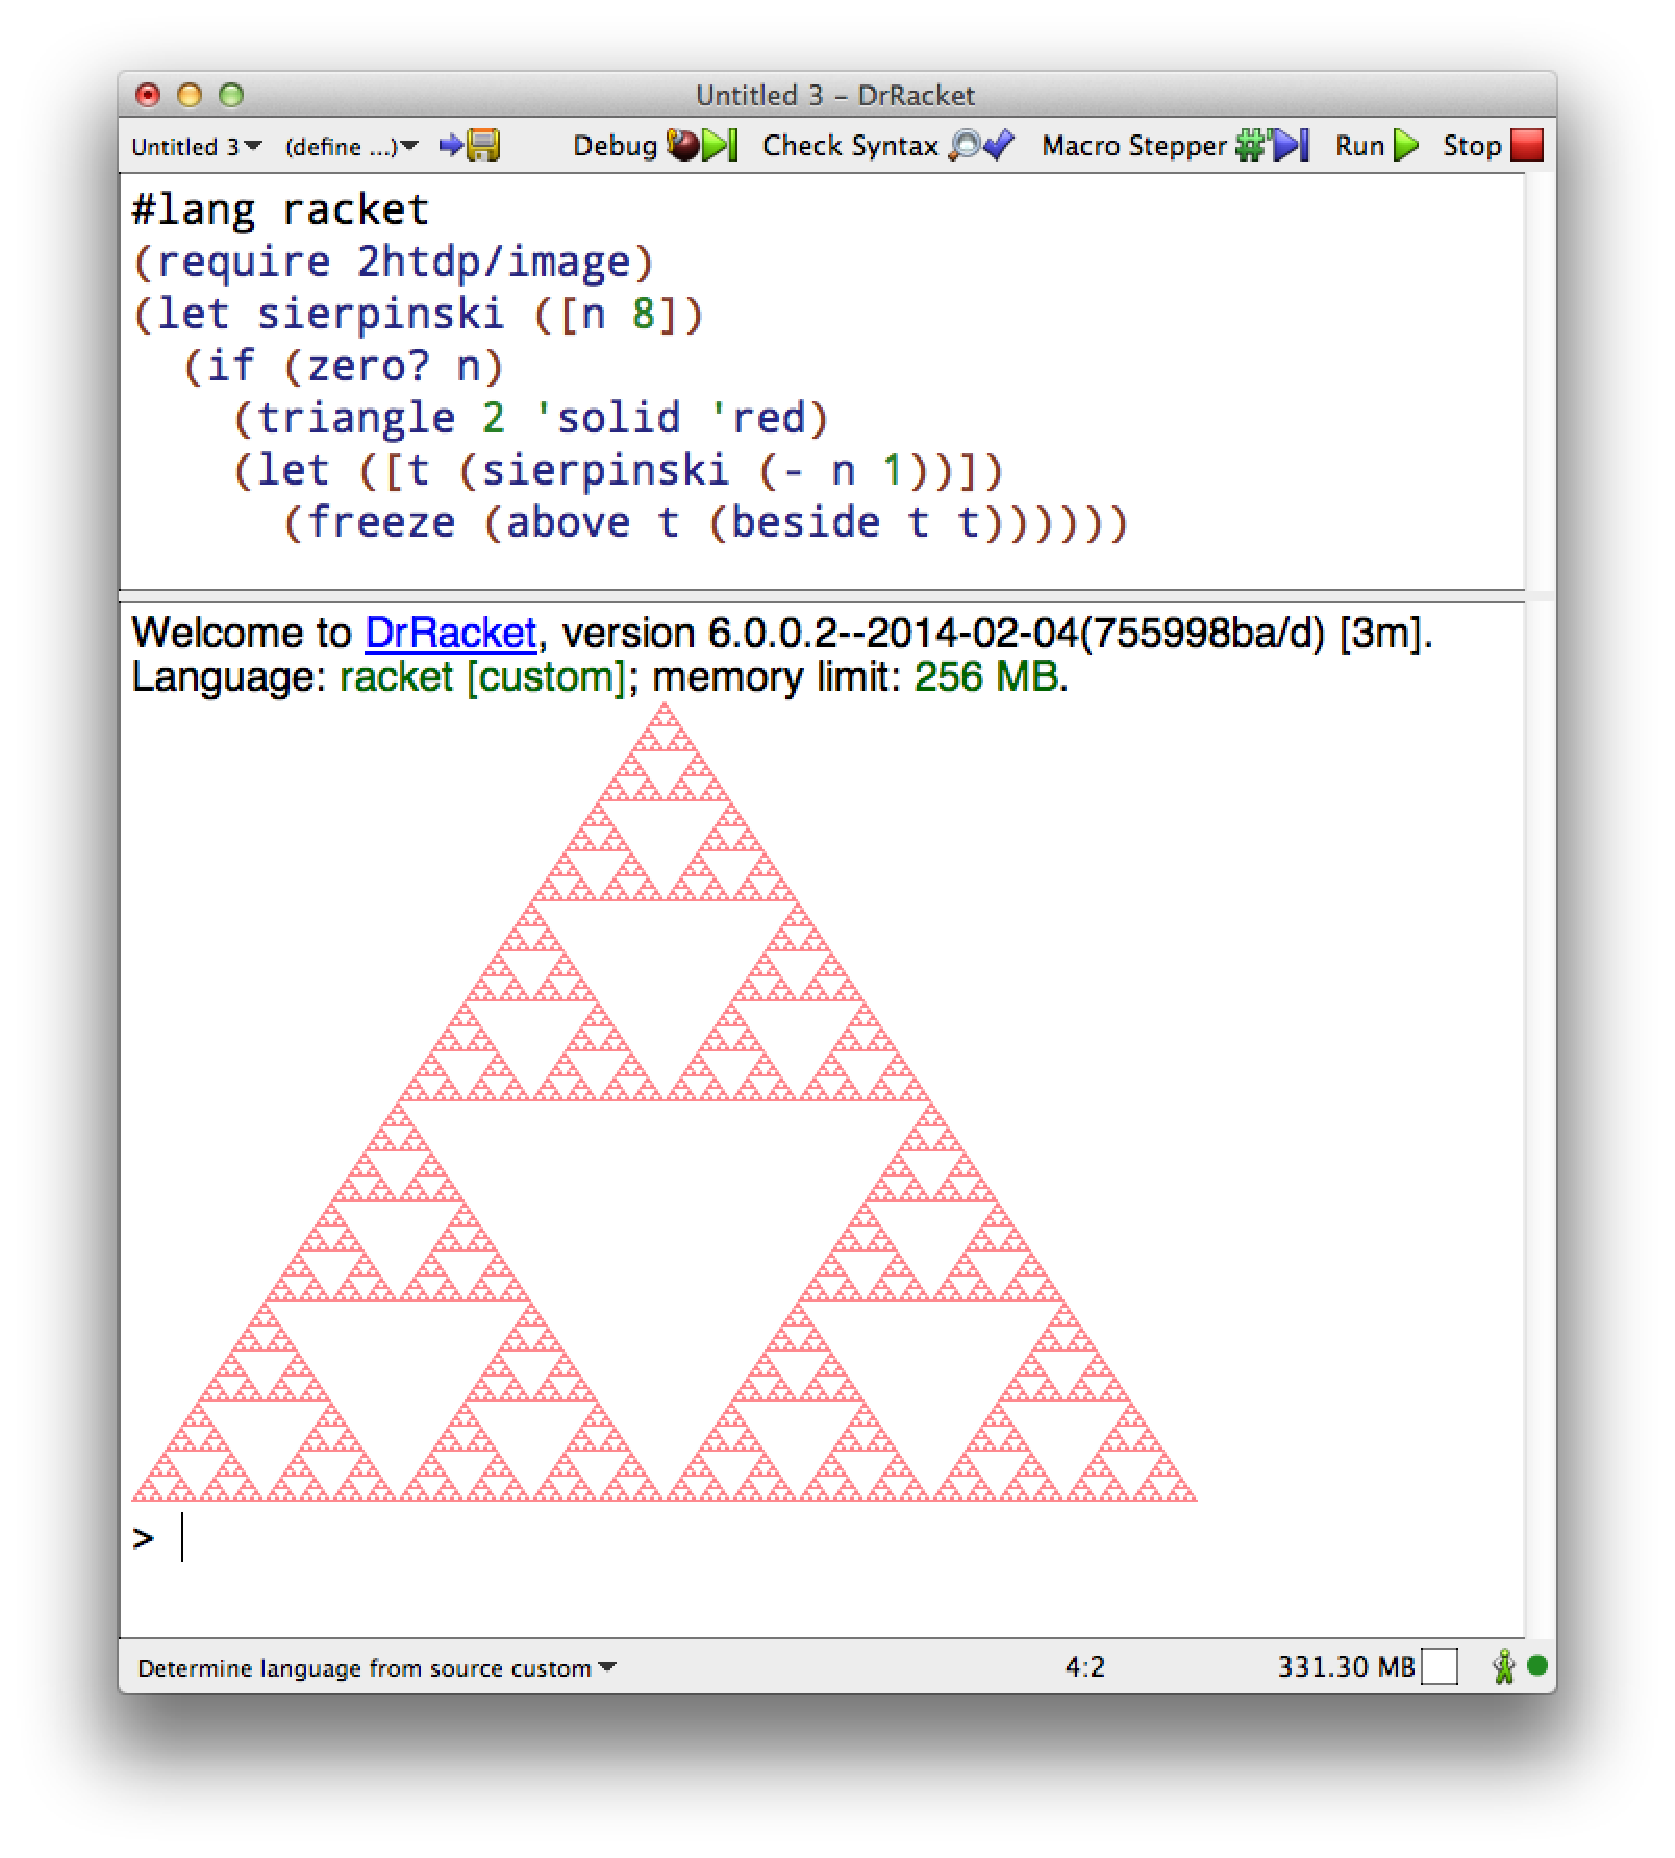
\includegraphics[width=5in]{figs/drracket}
\end{center}
\caption{The DrRacket interactive development environment.}
\label{fig:drracket}
\end{figure}


The interactions area has a prompt for accepting expressions to
evaluate.  Any definitions from the module are avaiable within the
interactions window, so we can experiment and calculate other results
of factorial:
\begin{verbatim}
> (fact (fact 5))
6689502913449127057588118054090372586752746333138029
8102956713523016335572449629893668741652719849813081
5763789321409055253440858940812185989848111438965000
5964960521256960000000000000000000000000000
\end{verbatim}

Changes that are made to the module are not immediately reflected in
the interactions window.  The program has to be re-run, which creates
a fresh interactions window, discarding anything you may have entered.
(But scrolling through a history of expressions is possible with
Cmd+Up.)


%% Because of this, the language incorporates an array of cutting edge PL
%% features for creating programming languages.  In fact, ``Racket'' is
%% not really a programming language, but a programming language
%% ecosystem.  Modules, which are the basic unit of code, can be written
%% in any of dozens of various languages

\subsection{Defining a Language}

To construct a Redex model of a language, the first thing to do is
declare the host language ({\tt racket}) and require the Redex
library:
\begin{verbatim}
#lang racket
(require redex)
\end{verbatim}

Defining the syntax of a language is accomplished with {\tt
  define-language}, which gives the grammar of terms for the language:
\begin{verbatim}
(define-language A
  (e ::= 
     v
     (Pred e)
     (Succ e)
     (Plus e e)
     (Mult e e))
  (v ::= i)
  (i j k ::= integer))
\end{verbatim}
This establishes the set of terms in the language {\tt A}, and also
establishes a number of meta-variable names which can be used to
pattern match terms.

For example, we can query the language to see if the term {\tt 4} is
in the set of values ranged over by meta-variable {\tt e}:
\begin{verbatim}
> (redex-match? A e (term 4))
#t
\end{verbatim}
It's also true that {\tt i} ranges over {\tt 4}:
\begin{verbatim}
> (redex-match? A i (term 4))
#t
\end{verbatim}
But while {\tt (Pred 4)} is in {\tt e}, it is not in {\tt i}:
\begin{verbatim}
> (redex-match? A e (term (Pred 4)))
#t
> (redex-match? A i (term (Pred 4)))
#f
\end{verbatim}

\subsection{Terms}

Terms in Redex are constructed with the {\tt term} form.  To a first
approximation, {\tt term} is just a synonym for {\tt quote}, which
constructs literal data.  In fact we could have constructed our
examples in the previous section with {\tt quote}, which can be written
{\tt (quote e)} or {\tt 'e} for short:
\begin{verbatim}
> (redex-match? A e '(Pred 4))
#t
> (redex-match? A i '(Pred 4))
#f
\end{verbatim}

The difference between {\tt term} and {\tt quote} is that {\tt term}
interprets some of the literal data.  The simplest example of this is
that {\tt term} interprets occurrences of bound meta-variables and
substitutes their values for the occurrences.  For example, we can
define a term variable with {\tt define-term} and then refer to it
within {\tt term} expressions:
\begin{verbatim}
> (define-term five 5)
> (term five)
5
> (quote five)
'five
\end{verbatim}
As we'll see, Redex comes with a powerful pattern matcher that let's
us match terms against term patterns and bind variables for use within
terms.

Another feature of {\tt term} is that it is possible to escape out of
the term language and back in to Racket.  This is accomplished with
{\tt unquote}.  The notation {\tt ,e} is a Racket shorthand for {\tt
  (unquote e)} and it signals to Redex not to interpret {\tt e} as a
term, but rather as a Racket expression which evaluates to a term.  In
other words.  Using the {\tt term} constructor within the expression
re-enters the Redex world, and this nesting can be arbitrarily deep.
Here are some examples:
\begin{verbatim}
> (term (Plus (add1 5)))
'(Plus (add1 5))
> (term (Plus ,(add1 5)))
'(Plus 6)
> (term (Plus ,(add1 (term five))))
'(Plus 6)
\end{verbatim}


\subsection{Defining a Reduction Relation}

A reduction relation is a value in Redex, constructed with the {\tt
  reduction-relation} form.  Defining the $\areducename$ relation is
achieved with:
\begin{verbatim}
(define a
  (reduction-relation
   A
   (--> (Pred i) ,(sub1 (term i)) pred)
   (--> (Succ i) ,(add1 (term i)) succ)
   (--> (Plus i j) ,(+ (term i) (term j)) plus)
   (--> (Mult i j) ,(* (term i) (term j)) mult)))
\end{verbatim}
A {\tt reduction-relation} specifies which language it operates on, in
this case {\tt A}.  The language determines the interpretation of the
meta-variables (and what whether a peice of syntax is a
meta-variable).  The relation is written as a set of axioms, each of
which has the form {\tt (--> $L\;R\;\mathit{name}$)} where $L$ is a
\deftech{pattern} and $R$ is a \deftech{template} and $\mathit{name}$
is an optional name for the rule.  Applying a reduction relation to a
term matches the term against each pattern and if the match is
succesful produces the template with each meta-variable replaced by
the corresponding substructure of the pattern match.

A reduction relation can be applied with {\tt apply-reduction-relation}:
\begin{verbatim}
> (apply-reduction-relation a (term (Pred 5)))
'(4)
\end{verbatim}
When the relation is not defined on a term, the empty list is produced:
\begin{verbatim}
> (apply-reduction-relation a (term (Mult (Pred 4) 5)))
'()
\end{verbatim}

There are a few operations on reduction relations that produce new
reduction relations.  For example, {\tt compatible-closure} computes
the compatible closure of a relation:
\begin{verbatim}
> (apply-reduction-relation (compatible-closure a A e)
                            (term (Mult (Pred 4) 5)))
'((Mult 3 5))
\end{verbatim}
Like any value, we can name this relation using {\tt define}:
\begin{verbatim}
(define ->a (compatible-closure a A e))
\end{verbatim}
The {\tt apply-reduction-relation*} function computes the set of
irreducible terms that are in the transitive closure of a given
relation:
\begin{verbatim}
> (apply-reduction-relation* ->a (term (Mult (Pred 4) 5)))
'(15)
\end{verbatim}

The {\tt traces} function will visualize the reduction semantics as a
graph of related terms.  For example,
\begin{verbatim}
> (traces ->a (term (Mult (Plus (Succ 2) (Mult 2 2)) (Plus 5 5))))
\end{verbatim}
will launch a window displaying the graph in figure~\ref{fig:graph}.
\begin{figure}
\begin{center}
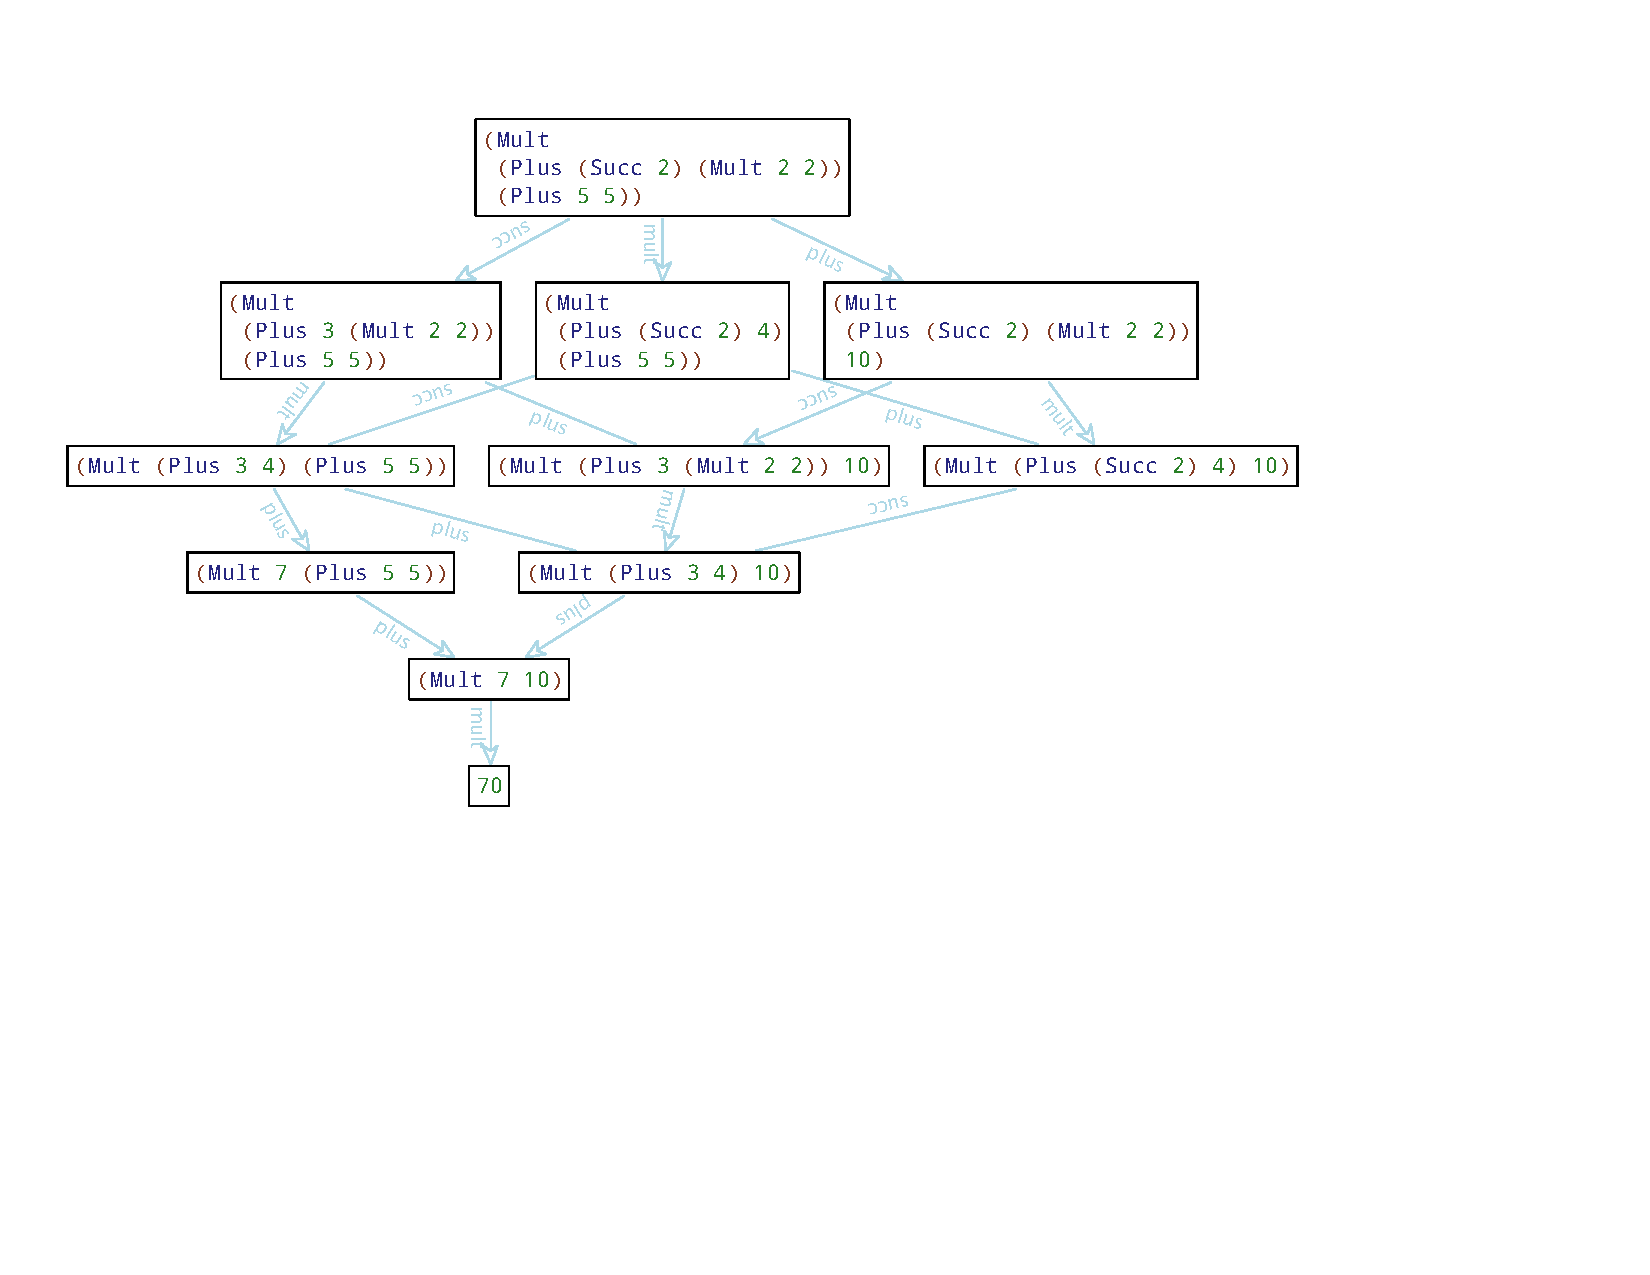
\includegraphics[width=5in]{figs/reduction-graph.pdf}
\end{center}
\caption{Example reduction graph.}
\label{fig:graph}
\end{figure}


\subsection{Defining metafunctions}

A metafunction is a function that is interpreted within the term
language.  Here is the natural semantics function written as a
metafunction in Redex:
\begin{verbatim}
(define-metafunction A
  [(eval v) v]
  [(eval (Pred e)) ,(sub1 (term (eval e)))]
  [(eval (Succ e)) ,(add1 (term (eval e)))]  
  [(eval (Plus e_1 e_2)) 
   ,(+ (term (eval e_1))
       (term (eval e_2)))]
  [(eval (Mult e_1 e_2))
   ,(* (term (eval e_1))
       (term (eval e_2)))])
\end{verbatim}

The function is defined by a series of pattern and template clauses,
much like a reduction relation but without the {\tt -->} notation.
Unlike a reduction relation, the patterns are tried in order and the
result of the metafunction application is the instantiated template of
the first matching clause.  An error is signalled if no clause
matches.

Once a metafunction is defined, it is applied whenever it occurs with
a {\tt term}:
\begin{verbatim}
> (term (eval (Mult (Pred 5) (Succ 8))))
36
> (term (Mult (Pred 5) (eval (Succ 8))))
'(Mult (Pred 5) 9)
\end{verbatim}

It's important to notice that this defines a \emph{function}, not a
\emph{relation}.  Since we know that $\Downarrow$ for $\Arith$ is a
function, this is a correct model of $\Downarrow$, but it would not be
if $\Downarrow$ were realy a relation, such as with the natural
semantics of imprecise errors for $\Barith$.  To model relations (that
are not reduction relations), we need another mecahnism: {\tt
  define-judgment-form}.

\subsection{Contexts}

Evaluation contexts can also be specified as part of a language's
grammar.  We can add the following to the {\tt define-language} for
{\tt A}:
\begin{verbatim}
  (E ::=
     hole
     (Pred E)
     (Succ E)
     (Mult E e)
     (Mult v E)
     (Plus E e)
     (Plus v E))
\end{verbatim}

Within a reduction relation and other patterns, {\tt in-hole} can be
used to match terms within a context.  For example, the standard
reduction relation can be defined as:
\begin{verbatim}
(define -->a
  (reduction-relation
   A
   (--> (in-hole E (Pred i)) (in-hole E ,(sub1 (term i))))
   (--> (in-hole E (Succ i)) (in-hole E ,(add1 (term i))))
   (--> (in-hole E (Mult i j)) (in-hole E ,(* (term i) (term j))))
   (--> (in-hole E (Plus i j)) (in-hole E ,(+ (term i) (term j))))))
\end{verbatim}

Since each of these rules has a repeated structure of using {\tt
  in-hole}, it's possible to define a shortcut:
\begin{verbatim}
(define -->a
  (reduction-relation
   A
   (~~> (Pred i) ,(sub1 (term i)))                                                              
   (~~> (Succ i) ,(add1 (term i)))                                                                   
   (~~> (Mult i j) ,(* (term i) (term j)))
   (~~> (Plus i j) ,(+ (term i) (term j)))
   with
   [(--> (in-hole E e_1) (in-hole E e_2))
    (~~> e_1 e_2)]))
\end{verbatim}
Or, we could simple compute the relation by using {\tt
  context-closure} and the existing reduction relation {\tt a}:
\begin{verbatim}
(define -->a
  (context-closure a A E))
\end{verbatim}

\subsection{Defining a Judgment (Relation)}

Defining a relation is accomplished with the {\tt
  define-judgment-form} notation:
\begin{verbatim}
(define-judgment-form A
  #:mode (evalr I O)
  [(evalr v v)]
  [(evalr e v)
   -----------
   (evalr (Pred e) ,(sub1 (term v)))]
  [(evalr e v)
   -----------
   (evalr (Succ e) ,(add1 (term v)))]  
  [(evalr e_1 v_1)
   (evalr e_2 v_2)
   ---------------
   (evalr (Plus e_1 e_2) ,(+ (term v_1) (term v_2)))]
  [(evalr e_1 v_1)
   (evalr e_2 v_2)
   ---------------
   (evalr (Mult e_1 e_2) ,(* (term v_1) (term v_2)))])
\end{verbatim}

A judgment is a relation that is being modelled computationally as a
function.  The {\tt \#:mode} keyword gives a mode specification which
declares which parts of the relation can be consider inputs ({\tt I})
and which parts can be considered outouts ({\tt O}), which can be
thought of as specifying which positions are inputs and outputs in
this function.

A judgment is used with {\tt judgment-holds} form.  It can be used in
two ways, the first is to check if the relation holds on particular
values.  So for example, we can check that {\tt (Succ (Succ 4))}
evaluates to {\tt 6} with:
\begin{verbatim}
> (judgment-holds (evalr (Succ (Succ 4)) 6))
#t
\end{verbatim}
It's also possible to compute the set of all values related to {\tt
  (Succ (Succ 4))} with:
\begin{verbatim}
> (judgment-holds (evalr (Succ (Succ 4)) v) v)
'(6)
\end{verbatim}
The set of related terms is given as a list of results (in case, it's
always a singleton list).

\subsection{From Judgements to Reduction Relations}

The Redex {\tt reduction-relation} form is tailored toward writing
relations as a set of axioms.  Most of the inductive parts of a
reduction relation are computed as contextual or compatible closures,
which use the grammar of contexts or terms to guide the induction.
This is often, but not always, what is needed.  In cases where a
reduction relation requires a more general set of inference rules, a
useful modeling strategy is to define the relation as a judgment and
then define a reduction relation in terms of the judgment.  As an
example, here is a model of the natural numbers and a formulation of
``$\geq$'' as a reduction relation using this strategy:
\begin{verbatim}
#lang racket
(require redex)

(define-language Natural
  (N ::= Z (S N)))

(define-judgment-form Natural
  #:mode (>= I O)
  [(>= N N)]
  [(>= N_0 N_1)
   ---------------
   (>= (S N_0) N_1)])

(define ->>= 
  (reduction-relation 
   Natural
   (--> N_0 N_1
        (judgment-holds (>= N_0 N_1)))))

(traces ->>= (term (S (S (S Z)))))
\end{verbatim}

Running the reduction relation on the example of 3 produces the
following graph:
\begin{center}
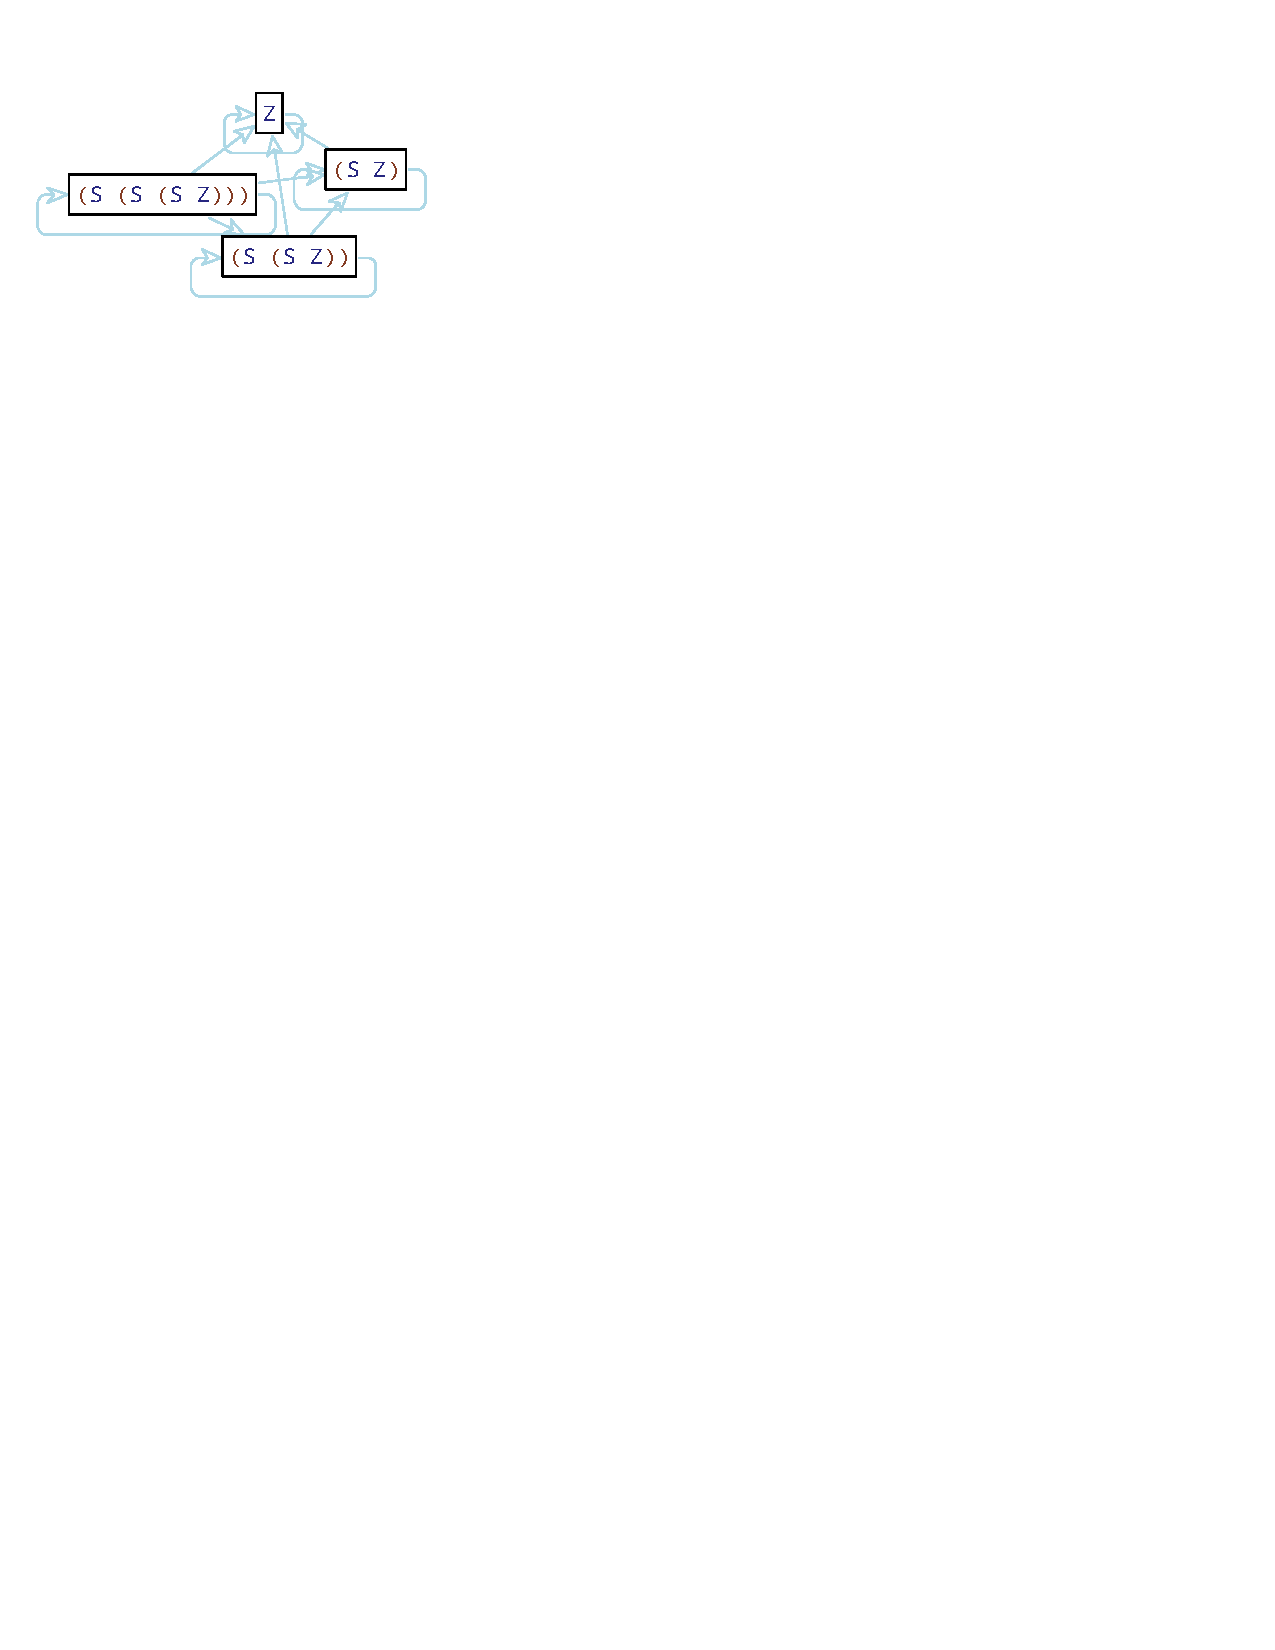
\includegraphics{figs/gte-graph.pdf}
\end{center}


\subsection{Property-Based Testing}

Semantic models are often buggy, just like programs.  One of the
easiest and quickest ways to test code is to state properties you
believe to be true and then test that the property holds for a bunch
of random inputs.

We believe the standard reductions semantics and natural semantics
correspond in the following way, for all {\tt e}:
\begin{verbatim}
  (equal? (apply-reduction-relation* -->a (term e))
          (judgment-holds (evalr e v) v))
\end{verbatim}
That is, for any term, the set of irreducible values reached by
iterating the standard reduction relation are exactly equal to the set
of values related by the natural semantics relation.  Redex will
generate random expressions and search for a counterexample with {\tt
  redex-check}:
\begin{verbatim}                                                                          
> (redex-check A e
               (equal? (apply-reduction-relation* -->a (term e))
                       (judgment-holds (evalr e v) v)))
redex-check: no counterexamples in 1000 attempts
\end{verbatim}
This generates 1000 random examples of {\tt e}s from the language {\tt
  A} and checks the expression, interpreted as a predicate universally
quantified over the pattern variable {\tt e}.  We can use arbitrary
patterns in place of {\tt e} to generate other kinds of data.

\subsection{Extending Languages}

Semantics engineers often start with small, simple models and grow
them over time into more realistic and rich languages.  We've seen
this with the development of $\Arith$ and $\Barith$ already.  Redex
supports exactly this kind of growth.

First, put the following at the top of the {\tt A} model and save it
in a file called {\tt A.rkt}.
\begin{verbatim}
(provide (all-defined-out))
\end{verbatim}

In another file, start with:
\begin{verbatim}
#lang racket
(require "A.rkt")
(require redex/reduction-semantics)
\end{verbatim}
This will import all of the defintions form the model for {\tt A}

We can now extend the syntax of {\tt A} to obtain {\tt B}:
\begin{verbatim}
(define-extended-language B A
  (e ::= ....
     x
     (Div e e)
     (Eq e e)
     (If e e e))
  (x ::= variable)
  (v ::= .... b)
  (b ::= True False) 
  (ρ ::= ((x v) ...))
  (E ::= ....
     (Div E e)
     (Div v E)
     (Eq E e)
     (Eq v E)
     (If E e e)))
\end{verbatim}
The ``{\tt e ::= ....}'' (that's \emph{four} dots) grammar means
everything that's an {\tt e} from {\tt A} plus the new productions
that follow.  It is really as if you had copied the grammar of {\tt e}
from {\tt A} in place of the ellipsis; all of the occurrences of the
non-terminal {\tt e}s in the grammar of {\tt A} range over {\tt e}s
drawn from {\tt B}.

The reduction relation {\tt a} can be lifted to work on {\tt B}
expressions and unioned with the new reduction axioms:
\begin{verbatim}
(define (b ρ)
  (union-reduction-relations 
   (extend-reduction-relation a B)
   (reduction-relation
    B
    (--> x v (where v (lookup ,ρ x)))
    (--> (Div i j) ,(quotient (term i) (term j))
         (side-condition (not (zero? (term j)))))    
    (--> (Eq i i) True)
    (--> (Eq i j) False
         (side-condition (not (= (term i) (term j)))))    
    (--> (If True e_1 e_2) e_1)
    (--> (If False e_1 e_2) e_2))))
\end{verbatim}
Note that this relation is indexed by an environment {\tt ρ}.
The {\tt lookup} metafunction looks up the value of a given
variable if it exists, or produced {\tt \#f}:
\begin{verbatim}
(define-metafunction B
  lookup : ρ x -> v or #f
  [(lookup ((x v) (x_0 v_0) ...) x) v]
  [(lookup ((x_0 v_0) (x_1 v_1) ...) x) 
   (lookup ((x_1 v_1) ...) x)]
  [(lookup () x) #f])
\end{verbatim}
The first line of this metafunction specifies a signature which states
it consumes an environment and variable and produces a value or {\tt
  \#f}.  It will result in an error if any of these conditions are
violated.  Although Redex doesn't have a type system, it's still
useful to catch these kinds of errors.

After the signature, there are three clauses, each consisting of a
pattern and a template.  The patterns are matched in order.  The first
clause matches when the first element in the environment contains the
variable {\tt x}, which is the same variable {\tt x} being looked up;
notice that the name {\tt x} is used twice in this pattern.  In this
case, {\tt lookup} produces the associated value from the environment.
The second clause matches when the environment is non-empty
and---knowing the first clause wasn't taken---the first element is not
what's being looked up.  In this case, {\tt lookup} looks up the
variable in the rest of the environment.  The third and final clause
matches when the environment is empty, meaning {\tt x} is not in the
environment.

A pattern of the form ``{\tt p ...}'' (that's \emph{three} dots!),
where {\tt p} is some pattern, means ``match {\tt p} zero or more
times.''  (You can think of it as Kleene star or ``$*$'' from regular
expressions.)  So the pattern {\tt (i ...)} matches {\tt ()}, {\tt
  (1)}, {\tt (1 2 3)}, etc.  So in the first clause of {\tt lookup}:
\begin{verbatim}
  [(lookup ((x v) (x_0 v_0) ...) x) v]
\end{verbatim}
This pattern matches an environment which starts with {\tt (x v)} and
then has zero or more {\tt (x\_0 v\_0)}s.  An easy mistake to make is to
write ``{\tt ...}'' as if it were a ``match anything'' pattern
signifying you don't care about the remaining data in the environment.
Thinking this way, you might instead write the clause as:
\begin{verbatim}
  [(lookup ((x v) ...) x) v]
\end{verbatim}
But this does not mean what you think it means.  The problem here is
we're matching many {\tt x}s since {\tt x} is part of the pattern
repeated by ``{\tt ...}'', and therefore we bind many {\tt v}s, but
the template only has one occurrence.  This kind of mismatch in number
will result in a syntax error complaining about a binder at different
depths.

Now let's look at the second clause:
\begin{verbatim}
  [(lookup ((x_0 v_0) (x_1 v_1) ...) x) 
   (lookup ((x_1 v_1) ...) x)]
\end{verbatim}
This pattern matches whenever the environment contains one or more
elements.  This is achieved by writing a pattern {\tt (x\_0 v\_0)} for
the one element and then {\tt (x\_1 v\_1) ...} for the remaining zero
or more elements.  This is a fairly common idiom for matching the
first and rest of a list.  The result calls {\tt lookup} with a
structurally smaller environment.


Programming with Redex's souped-up pattern matcher takes some getting
used to.  Try things out.  Make conjectures with test cases.

\begin{exercise} 
Design a metafunction {\tt pukool} which is like {\tt lookup} but
searches through the environment from right to left.  The following
test cases demonstrate the difference:
\begin{verbatim}
(test-equal (term (lookup ((x 1) (x 5)) x))
            (term 1))
(test-equal (term (pukool ((x 1) (x 5)) x))
            (term 5))
\end{verbatim}
\end{exercise}


We can further develop the semantics for errors as a further
extension:
\begin{verbatim}
(define-extended-language BE B
  (e ::= .... r)
  (r ::= (Err variable))
  (a ::= v r))
 
(define err
  (reduction-relation 
   BE
   (--> (Div i 0) (Err Div0))
   (--> (Div b v) (Err Div1))
   (--> (Div v b) (Err Div2))
   (--> (Eq b v) (Err Eq1))
   (--> (Eq v b) (Err Eq2))
   (--> (If i e_1 e_2) (Err If))))

(define prop
  (reduction-relation
   BE
   (--> (Pred r) r)
   (--> (Succ r) r)
   (--> (Plus r e) r)
   (--> (Plus v r) r)
   (--> (Mult r e) r)
   (--> (Mult v r) r)
   (--> (Div r e) r)
   (--> (Div v r) r)    
   (--> (Eq r e) r)
   (--> (Eq v r) r)
   (--> (If r e_0 e_1) r)))

(define (bep ρ)
  (union-reduction-relations 
   (extend-reduction-relation (b ρ) BE)
   err prop))
\end{verbatim}

\newcommand\typevaljudge[3]{{#1}\vdash{#2}:{#3}}
\newcommand\mtype{t}
\newcommand\typeof{\mathit{typeof}}
\newcommand\treduce{\mathbf{t}}
\newcommand\mtans{ta}
\newcommand\Ans{\mathit{Ans}}
\newcommand\TyAns{\mathit{TyAns}}

\newcommand\meint{i^\dagger}
\newcommand\moeint{j^\dagger}
\newcommand\mintv{\vec\mint}
\newcommand\mointv{\vec\moint}

\newcommand\BI{\mathcal{BI}}
\newcommand\ireduce{\mathbf{i}}
\newcommand\intvdiv{\mathop\backslash}

\section{Proving the Absence of (Certain Kinds of) Errors}

It would be nice to eliminate all programs that have errors in them.
In general, it's not possible to mechanically determine if a program
will cause an error when run, so much of program analysis, which is
the study of approximations to program properties, is concerned with
detecting or proving the absense of errors in programs.  One of the
most common forms of this kind of program analysis are \deftech{type
  systems}:

\begin{quotation}
A type system is a tractable syntactic method for proving the absence
of certain program behaviors by classifying phrases according to the
kinds of values they compute.

\raggedleft --- Benjamin C.~Pierce
\end{quotation}

In its simplest form, a type system can prove the absence of errors
that arise from applying operations to the wrong kinds of values.  Like
any program analysis, the classification of programs into those that
have these kind of errors and those that do not must be approximate.
So the classification will err on the side of caution and classify
programs as \emph{definitely} not having this kinds of errors or
\emph{potentially} having them.  In other words, a type system will
misclassify some good programs as bad, but no bad program will be
classified as good.


\subsection{Type Judgments}\label{sec:type-judgments}

In the language of $\Barith$ expressions, there are two kinds of data:
Booleans and integers.  We can formalize a judgment on programs that
classifies them according to the data they produce, eliminating the
possibility of errors arising from misusing data.

A type is either $\Bool$ or $\Int$:
\[
\begin{array}{llcl}
\mathit{Type} & \mtype & = & \Bool\ |\ \Int
\end{array}
\]

A \deftech{type judgment} is a ternary relation on environments,
expressions, and types:
\[
\typevaljudge\menv\mexp\mtype
\]
If a program $(\menv,\mexp)$ is related to $\mtype$ it means the
program evaluates to some value of that type:
\begin{align*}
\typevaljudge\menv\mexp\Int \Rightarrow \beval\menv\mexp\mint\\
\typevaljudge\menv\mexp\Bool \Rightarrow \beval\menv\mexp\mbool
\end{align*}
Thus the relation captures a class of well-behaved programs that do no
cause type errors.  The natural semantics employed here could either
be the one that considers erroneous programs meaningless or the
explicit error semantics.

There is a small wrinkle here having to do with divide-by-zero errors,
and even without seeing the definition of the relation, you may be
(rightfully) doubting the above claims.  Let us punt on the wrinkle
for now and consider $\Div$ banished from $\Barith$ (we will restore
it later).

At first approximation, you might think of the ``$:$'' as a strange
kind of evaluation relation, which gives an approximation of the
``real'' relation ``$\Downarrow$.''  Instead of saying exactly what an
expression evaluates to, the ``:'' says what set of values the result
belongs to.  That intuition can guide the definition of the relation.
So for example, an integer expression evaluates to something in
$\Int$, and a Boolean evaluates to someting in $\Bool$:
\begin{mathpar}
\inferrule{\ }
          {\typevaljudge\menv\mint\Int}

\inferrule{\ }
          {\typevaljudge\menv\mbool\Bool}
\end{mathpar}
Likewise, variables bound to integers and Booleans behave similarly:
\begin{mathpar}
\inferrule{\menv(\mvar) = \mint}
          {\typevaljudge\menv\mvar\Int}

\inferrule{\menv(\mvar) = \mbool}
          {\typevaljudge\menv\mvar\Bool}
\end{mathpar}
If an expression $\mexp$ evaluates to something in $\Int$, so does
$\Succ(\mexp)$ and $\Pred(\mexp)$:
\begin{mathpar}
\inferrule{\typevaljudge\menv\mexp\Int}
          {\typevaljudge\menv{\Pred(\mexp)}\Int}

\inferrule{\typevaljudge\menv\mexp\Int}
          {\typevaljudge\menv{\Succ(\mexp)}\Int}
\end{mathpar}
If expressions $\mexp_1$ and $\mexp_2$ evaluate to values in $\Int$,
then $\Plus(\mexp_1,\mexp_2)$ and $\Mult(\mexp_1,\mexp_2)$ evaluate to
values in $\Int$ and $\Eq(\mexp_1,\mexp_2)$ evaluates to values in
$\Bool$:
\begin{mathpar}
\inferrule{\typevaljudge\menv{\mexp_1}\Int \\
           \typevaljudge\menv{\mexp_2}\Int}
          {\typevaljudge\menv{\Plus(\mexp_1,\mexp_2)}\Int}

\inferrule{\typevaljudge\menv{\mexp_1}\Int \\
           \typevaljudge\menv{\mexp_2}\Int}
          {\typevaljudge\menv{\Mult(\mexp_1,\mexp_2)}\Int}

\inferrule{\typevaljudge\menv{\mexp_1}\Int \\
           \typevaljudge\menv{\mexp_2}\Int}
          {\typevaljudge\menv{\Eq(\mexp_1,\mexp_2)}\Bool}
\end{mathpar}
Finally, there is the matter of $\If$.  It's clear that the test
expression $\If(\mexp_1,\mexp_2,\mexp_3)$ should evaluate to some
value in $\Bool$, but what should the whole expression evaluate to?
If all we know of $\mexp_1$ is it evaluates to a Boolean, then the
whole expression either evaluates to the value of $\mexp_1$ or
$\mexp_2$.  But which is it?  One approach is to require $\mexp_1$ and
$\mexp_2$ to evaluate to values within the same set.  You've probably
encountered this before: both branches of an $\If$ must have the same
type.  Adopting this approach, the rule is:
\begin{mathpar}
\inferrule{\typevaljudge\menv{\mexp_1}\Bool\\
           \typevaljudge\menv{\mexp_2}\mtype\\
           \typevaljudge\menv{\mexp_3}\mtype}
          {\typevaljudge\menv{\If(\mexp_1,\mexp_2,\mexp_3)}\mtype}
\end{mathpar}

Now we have a typing relation, although it's not exactly clear what we
have gained.  After all, we could have just run a program to discover
if it caused an error.  That said, it still may be cheaper, even for
this simple type system, to compute the type than to compute the
evaluation.  As our language grows, the gap between the resources
required to run and analyze a program can grow without bound, so this
point shouldn't be entirely disregarded.  However, the real value of
this system comes into play after making the following observation:
the environment plays no role in the type relation other than to
signify the types of variables by supplying a witness to the type.
In other words, in the typing derivation of
\[
\typevaljudge{[\mathit{x}\mapsto 4]}{\If(\Eq(\mathit{x},7),\False,\True)}{\Bool}
\]
it doesn't matter at all that $\mathit{x}$ is bound to $4$ in
particular.  Any integer would have sufficed to prove this program
produces a Boolean.  Intuitively, we can make a much stronger claim
about this program, which is that on any integer input, the program
does not produce an error.  By reasoning about a single ``abstract''
run of the program, we can conclude facts about all possible
``concrete'' runs: none of them produce errors.

We can make this claim precise with a relation on environments.  
First, let's define:
\begin{align*}
\typeof(\mint) = \Int\\
\typeof(\mbool)= \Bool
\end{align*}
Two environments ``agree,'' written $\menv \sim \menv'$ when they map
variables to values of the same type:
\begin{mathpar}
\inferrule
{\forall \mvar \in \dom(\menv) . \typeof(\menv(\mvar)) = \typeof(\menv'(\mvar))}
{\menv \sim \menv'}
\end{mathpar}

\begin{claim}
If $\typevaljudge\menv\mexp\mtype$ and $\menv \sim \menv'$, then 
$\typevaljudge{\menv'}\mexp\mtype$.
\end{claim}
\begin{proof}
By structural induction on the derivation of $\typevaljudge\menv\mexp\mtype$.  The
integer and Boolean cases are trivial.  The variable cases follow from
the definition of $\sim$.  The remaining cases follow by induction.
\end{proof}

Since the environment really only informs the system of the type of
each variable, we can replace the value environment with a
\deftech{type environment} that directly maps a variable to its type.
We use the metavariable $\Gamma$ to range over type environments.  The
type judgment is obtained simply by replacing $\menv$ with $\Gamma$ in
all the rules except the variable rules, which are replaced with:
\begin{mathpar}
\inferrule{\Gamma(\mvar) = \mtype}
          {\typevaljudge\Gamma\mexp\mtype}
\end{mathpar}
%
We can extend the ``$\sim$'' relation to relate type environments and
value environments:
\begin{mathpar}
\inferrule
{\forall \mvar \in \dom(\Gamma) . \Gamma(\mvar) = \typeof(\menv(\mvar)) }
{\Gamma \sim \menv}
\end{mathpar}
The soundness of the typing judgment formalizes our understanding of
the classification of programs into those that do not produce errors
and those that may:
\begin{claim}
If $\typevaljudge\Gamma\mexp\mtype$ and $\Gamma \sim \menv$, then
$\beval\menv\mexp\mval$ and $\typeof(v) = t$.
\end{claim}
\begin{proof}
By structural induction on the derivation of $\typevaljudge\Gamma\mexp\mtype$.
\end{proof}

Type systems are arguably the most effective and widely used formal
verification tool in use today.  In the development above, we've come
up with a fairly simple type system that can prove the absence of
certain errors in programs.  In our case, the class of errors is
simple; it rules out errors arising from branching on non-Booleans and
applying numeric operators to non-numeric arguments.  Much of the work
in developing type systems has been in developing richer notions of
errors and corresponding type judgements that safely classify error
free programs.  But every type system must necessarily throw good
programs out with the bad.  For example, this type system rejects the
following error free programs:
\begin{align*}
\If(\mathit{x},7,\False)\mbox{, where $\mathit{x}:\Bool$}\\
\If(\False,\Eq(\True,1),7)\\
\If(\mathit{x},\If(\mathit{x},7,\Eq(\True,1)),8)\mbox{, where $\mathit{x}:\Bool$}
\end{align*}

\paragraph{Note on Runtime Errors:} 
Type systems often only rule out a certain class of errors.  Which
class depends on the particular type system.  The system we've just
developed rules out all errors except $\Err_{\Div0}$ errors, which
were ommitted from the presentation for simplicity.  To be precise
about divide-by-zero errors would require some tedious and
uninteresting additions to the semantics and conditions on the claims.


\subsection{Abstract Interpretation with Types}\label{sec:ai-types}

In this section, let's take an alternative perspective on the type
judgement of the previous section.  If ``$:$'' is a funny analog of
``$\Downarrow$'', a natural question is what is the reduction
semantics equivalent of ``$:$''?

First, let's embed types in the language of $\Barith$ expressions:
\[
\begin{array}{llcl}
  & \mexp & ::= & \dots\ |\ \mtype
\end{array}
\]

The reduction axioms are easy to read-off from the typing judgement:
\begin{mathpar}
\inferrule{\ }
          {\envreduce[\Gamma]\mint\treduce\Int}

\inferrule{\ }
          {\envreduce[\Gamma]\mbool\treduce\Bool}

\inferrule{\Gamma(\mvar) = \mtype}
          {\envreduce[\Gamma]{\mvar}\treduce\mtype}

\inferrule{\ }
          {\envreduce[\Gamma]{\Pred(\Int)}\treduce\Int}

\inferrule{\ }
          {\envreduce[\Gamma]{\Succ(\Int)}\treduce\Int}

\inferrule{\ }
          {\envreduce[\Gamma]{\Plus(\Int,\Int)}\treduce\Int}

\inferrule{\ }
          {\envreduce[\Gamma]{\Mult(\Int,\Int)}\treduce\Int}

\inferrule{\ }
          {\envreduce[\Gamma]{\Eq(\Int,\Int)}\treduce\Bool}

\inferrule{\ }
          {\envreduce[\Gamma]{\If(\Bool,\mtype,\mtype)}\treduce\mtype}
\end{mathpar}
We can define $\compat\treduce$ as the compatible closure of
$\treduce$ over the grammar of expressions and $\multicompat\treduce$
as the reflexive, transitive closure of $\compat\treduce$.  Analogs of
the type soundness property hold in this system, too.
\begin{claim}
\label{claim:reduce-soundness}
If $\envreduce[\Gamma]\mexp{\multicompat\treduce}\mtype$ and
$\Gamma\sim\menv$, then
$\envreduce\mexp{\multicompat\breducename}\mval$ and $\typeof(\mval)=\mtype$.
\end{claim}
\begin{exercise}
Prove claim \ref{claim:reduce-soundness}.
\end{exercise}

More than just a change of notation, the reduction semantics view
opens up some new design possibilities.  For example, the $\If$ axiom
requires both branches to be reduced to (abstract) values, i.e.~types,
before proceeding.  What if we mimicked the original semantics more
closely and replace the $\If$ rule with the following:
\begin{mathpar}
\inferrule{\ }
          {\envreduce[\Gamma]{\If(\Bool,\mexp_1,\mexp_2)}{\treduce'}{\mexp_1}}

\inferrule{\ }
          {\envreduce[\Gamma]{\If(\Bool,\mexp_1,\mexp_2)}{\treduce'}{\mexp_2}}
\end{mathpar}

While the above is a more precise abstraction of the $\breducename$
semantics, it leads to some potentially undesirable properties.  The
semantics are not consistent and claim~\ref{claim:reduce-soundness} is
not true.  Consider the example from earlier:
\[
\If(\mathit{x},7,\False)\text{, where }\mathit{x}:\Bool
\]
In the $\treduce'$ semantics, this program reduces to both $\Int$ and
$\Bool$.

\begin{exercise}
Construct a counterexample to claim~\ref{claim:reduce-soundness} for $\treduce'$.
\end{exercise}

The $\multicompat{\treduce'}$ semantics, however, does offer some
strong guarantees.  In particular, the semantics is useful for
informing us of what the program \emph{does not evaluate to}.  If
ruling out behaviors such as type errors is all we care about, this is
just as useful as the previous system which informed of us of what the
program does evaluate to.  After all, saying a program always
evaluates to an integer is a way of saying what it does not evaluate
to, also.

So we can formalize this with the following claim:
\begin{claim}\label{claim:neg-soundness-small}
If $\neg(\envreduce[\Gamma]\mexp{\multicompat{\treduce'}}\mtype)$ and $\Gamma\sim\menv$, then
$\neg(\envreduce\mexp{\multicompat{\breducename}}\mval)$ where $\typeof(\mval)=\mtype$.
\end{claim}
While true, this negative formulation doesn't quite let us conclude
that some programs are error free.  The solution is to again mimick
the original semantics more closely and explicitly characterize the
error behavior of programs.

Suppose we add rules corresponding the axioms for creating and
propogating errors (only showing a small excerpt):
\begin{mathpar}
\inferrule{\mtype \neq \Bool}
          {\envreduce[\Gamma]{\If(\mtype,\mexp_1,\mexp_2)}{\treduce'}{\Err_{\If0}}}

\inferrule{\ }
          {\envreduce[\Gamma]{\If(\merr,\mexp_1,\mexp_2)}{\treduce'}{\merr}}

\inferrule{\ }
          {\envreduce[\Gamma]{\Eq(\merr,\mexp)}{\treduce'}\merr}

\inferrule{\ }
          {\envreduce[\Gamma]{\Eq(\mtype,\merr)}{\treduce'}\merr}
\end{mathpar}
Programs now reduce to a type or an error, which we'll call a type answer:
\[
\begin{array}{llcl}
\mathit{TyAns}  & \mtans & ::= & \mtype\ |\ \merr
\end{array}
\]
We need to relate type answers and answers, which we do by a
relation $\mans \sqsubseteq \mtans$:
\begin{mathpar}
\inferrule{\typeof(\mval) = \mtype}
          {\mval \sqsubseteq \mtype}

\inferrule{\ }
          {\merr \sqsubseteq \merr}
\end{mathpar}
We can now state a generalization of claim~\ref{claim:neg-soundness-small}:
\begin{claim}\label{claim:neg-soundness}
If $\neg(\envreduce[\Gamma]\mexp{\multicompat{\treduce'}}\mtans)$ and $\Gamma\sim\menv$, then
$\neg(\envreduce\mexp{\multicompat{\breducename}}\mans)$ where $\mans \sqsubseteq \mtans$.
\end{claim}
We can also state this claim in an equivalent way which says that if a
program can evaluate to some answer, then an appoximation of that
answer is in the abstract evaluation of the program:
\begin{claim}[Soundness]\label{claim:soundness}
If $\envreduce\mexp{\multicompat{\breducename}}\mans$ and
$\Gamma\sim\menv$, then
$\envreduce[\Gamma]\mexp{\multicompat{\treduce'}}\mtans$ where $\mans
\sqsubseteq \mtans$.
\end{claim}
\begin{exercise}
Prove claim~\ref{claim:soundness}.
\end{exercise}

The above formulation let's us talk about error-freedom in a more
refined way since we can say exactly what kind of errors a program may
or may not have.  In fact, it's easy now to deal with divide-by-zero
errors by including reduction axioms for $\Div$:
\begin{mathpar}
\inferrule{\ }
          {\envreduce[\Gamma]{\Div(\Int,\Int)}{\treduce'}{\Int}}

\inferrule{\ }
          {\envreduce[\Gamma]{\Div(\Int,\Int)}{\treduce'}{\Err_{\Div0}}}
\end{mathpar}
The case on the right may seem unfortunate because it says that
\emph{any} program that includes a $\Div$ operation which may be
evaluated can cause a divide-by-zero error, including things like
$\Div(12,4)$.  But that's no different that the guarantee OCaml gives
you when it says an expression is of type {\tt int}.  In the system
above, at least we can say that if an expression does not (abstractly)
reduce to $\Err_{\Div0}$, then it definitely cannot produce a
divide-by-zero error.

The development of the reduction-based formulation of type system is
an instance of \deftech{abstract interpretation}.  And in fact, the
original type judgement can be seen as a further abstract
interpretation of the reduction semantics.  Abstract interpretation
(AI) is a general theory of semantic approximation.  Therefore it
serves as a good foundation for the theory of static analysis since
static analysis consists of computable semantic approximations.  (AI
is also useful beyond static analysis as it can be used to related
different forms of semantics such as natural semantics and reduction
semantics.)

%% The theory of abstract interpretation is grounded in the theory of
%% lattices and Galois connections, which relates two partially ordered
%% sets.  Before studying AI in detail though, let's just develop another
%% example to gain intuitions.


\subsection{Abstract Interpretation with Intervals}\label{sec:ai-intv}

In this section, let's develop another abstract interperation of
$\Barith$, this time with a more refined abstract domain.  On
integers, we'll use intervals and interpret the integer operations
using interval arithmetic and on Booleans we'll do no approximation.
Intervals will be represented as a pair of extended integers,
i.e. integers extended with ``$\infty$'' and ``$-\infty$''.  We'll use
$\meint$ and $\moeint$ to range over extended integers and $\mintv$
and $\mointv$ to range over intervals, i.e. pairs of extended integers
$(\meint,\moeint)$ where we assume $\meint$ is either $-\infty$ or an
integer and $\moeint$ is either $\infty$ or an integer.  An interval
is interpreted as a non-empty set of integers in the following way:
\begin{align*}
(-\infty,\infty) &= \mathbb{Z}\\
(-\infty,\moint) &= \{ \mint'\ |\ \mint' \leq \moint \}\\
(\mint,\infty) &= \{ \mint'\ |\ \mint \leq \mint' \}\\
(\mint,\moint) &= \{ \mint'\ |\ \mint \leq \mint' \leq \moint \}
\end{align*}

We define the $\BI$ language as $\Barith$, but with intervals in place
of integers in the set of values:
\[
\begin{array}{llcl}
\mathit{Exp}  & \mexp & ::= & \dots\ |\ \mint\ |\ \mintv\\
\mathit{Val}  & \mval & ::= & \mintv\ |\ \mbool
\end{array}
\]

Instead of a type environment as used in $\treduce$, we'll let
$\Gamma$ range over interval environments that map variables to
intervals (or Booleans).
%
The reduction axioms are easy in many cases:
\begin{mathpar}
\inferrule{\ }
          {\envreduce[\Gamma]\mint\ireduce(\mint,\mint)}

\inferrule{\Gamma(\mvar) = \mval}
          {\envreduce[\Gamma]\mvar\ireduce\mval}

\inferrule{\ }
          {\envreduce[\Gamma]{\Pred(\mintv)}\ireduce{\mintv - (1,1)}}

\inferrule{\ }
          {\envreduce[\Gamma]{\Succ(\mintv)}\ireduce{\mintv + (1,1)}}

\inferrule{\ }
          {\envreduce[\Gamma]{\Plus(\mintv,\mointv)}\ireduce{\mintv + \mointv}}

\inferrule{\ }
          {\envreduce[\Gamma]{\Mult(\mintv,\mointv)}\ireduce{\mintv \cdot \mointv}}

\inferrule{\ }
          {\envreduce[\Gamma]{\If(\True,\mexp_1,\mexp_2)}\ireduce{\mexp_1}}

\inferrule{\ }
          {\envreduce[\Gamma]{\If(\False,\mexp_1,\mexp_2)}\ireduce{\mexp_2}}
\end{mathpar}
These definitions make use of extended interval arithmetic operations
``$+$'', ``$-$'', and ``$\cdot$''.  Interval arithmetic is well
understood mathematical domain, and these operations can be
illustrated with just a few examples:
\begin{align*}
(1,5)+(3,9) &= (1,14)\\
(2,5)\cdot(3,9) &= (6,45)\\
(-\infty,5)\cdot(3,9) &= (-\infty,45)
\end{align*}

Things get trickier with equality.  Because an interval represents a
set of potential integer values, $\Eq(\mintv,\mointv)$ must produce
$\True$ whenever there are two equal integers in the sets denoted by
$\mintv$ and $\mointv$ and $\False$ whenever there are two unequal
integers in the sets.
\begin{mathpar}
\inferrule{\exists\mint\in\mintv.\exists\moint\in\mointv.\mint=\moint}
          {\envreduce[\Gamma]{\Eq(\mintv,\mointv)}\ireduce{\True}}

\inferrule{\exists\mint\in\mintv.\exists\moint\in\mointv.\mint\neq\moint}
          {\envreduce[\Gamma]{\Eq(\mintv,\mointv)}\ireduce{\False}}
\end{mathpar}
These definitions give the most precise relation our interval
abstraction allows; i.e. this is the best approximation possible
without changing the domain.  The preconditions form a good
specification, but clearly an implementation should not enumerate the
(potentially infinite) integers in $\mintv$ and $\mointv$ to check the
for (in-)equality.  Instead, produce $\True$ whenever $\mintv$ and
$\mointv$ overlap at all.  Determining when to produce $\False$
requires a little more thought.  You want to produce $\False$ almost
all the time.  When should $\False$ not be one of the results?

Things get even trickier with division.  First, here are some examples
of integer division on intervals:
\begin{align*}
(12,24)\mathop\backslash(3,4) &= (3,8)\\
(12,24)\mathop\backslash(3,\infty) &= (0,8)\\
(12,\infty)\mathop\backslash(3,\infty) &= (0,\infty)
\end{align*}
Interval division is not defined when $0$ is in the denominator
interval.

It's tempting to define $\ireduce$ for $\Div$ as the following:
\begin{mathpar}
\inferrule{0 \not\in \mointv}
          {\envreduce[\Gamma]{\Div(\mintv,\mointv)}\ireduce{\mintv \mathop{\backslash} \mointv}}

\inferrule{0 \in \mointv}
          {\envreduce[\Gamma]{\Div(\mintv,\mointv)}\ireduce{\Err_{\Div0}}}
\end{mathpar}
But this definition is not sound.  To see why, let's formalize the
soundness property.  Again, it will be in terms of a refinement
relation between answers of $\Barith$ and $\BI$:
\begin{mathpar}
\inferrule{\mint \in \mintv}
          {\mint \sqsubseteq \mintv}

\inferrule{\ }
          {\merr \sqsubseteq \merr}

\inferrule{\ }
          {\mbool \sqsubseteq \mbool}
\end{mathpar}
This relation is lifted to environments as usual:
\begin{mathpar}
\inferrule{\forall \mvar \in \dom(\menv) . \menv(\mvar) \sqsubseteq \Gamma(\mvar)}
          {\menv \sqsubseteq \Gamma}
\end{mathpar}
Assuming $\multicompat\ireduce$ is the reflexive transitive closure of
the compatible closure of $\ireduce$, the soundness claim is then:
\begin{claim}[Soundness]\label{claim:intv-soundness}
If $\envreduce\mexp{\multicompat{\breducename}}\mans$ and
$\menv \sqsubseteq \Gamma$, then
$\envreduce[\Gamma]\mexp{\multicompat{\ireduce}}\mans'$ where $\mans
\sqsubseteq \mans'$.
\end{claim}
\begin{exercise}
Construct a counterexample to claim~\ref{claim:intv-soundness} using
the faulty definition of $\ireduce$ for $\Div$.
\end{exercise}

\begin{exercise}
Design the best sound alternative of $\ireduce$ for $\Div$.
By sound, it should validate claim~\ref{claim:intv-soundness};
by best, it should be the smallest relation that does so.
\end{exercise}

\subsection{Refinement Types}

In section~\ref{sec:type-judgments} we developed a simple type system
that ruled out type errors.  By viewing the typing judgement as a
approximate evaluation relation, we explored an equivalent formulation
of the type system as an approximate reduction relation in
section~\ref{sec:ai-types}.  We then revealed a more precise semantics
for proving the absence of type errors.  In section~\ref{sec:ai-intv},
we developed an interval abstraction of the reduction semantics for
$\Barith$.  We can also go in the opposite direction and derive a
further approximation of the interval abstraction in the form of a
natural semantics.  This semantics takes the form of a type judgment,
where the the language of types is refined by an interval in the case
of integers:
\[
\begin{array}{llcl}
\mathit{Type}  & \mtype & ::= & \Bool\ |\ \Int(\mintv)
\end{array}
\]

The type $\Int(\mintv)$ is known as a \deftech{refinement type}, which
is a type qualified by a predicate which holds for every value of that
type.  For our purposes, the predicates only include intervals, but
richer refinement type systems can be defined by embeding richer
logics of predicates into the types.  Refinement types, while not
quite mainstream yet, are featured in several mature research project
such as the refinement type system for F\# called
F7\footnote{\url{http://research.microsoft.com/en-us/projects/f7/}}
and a variant of Haskell with refinements called Liquid
Haskell\footnote{\url{http://goto.ucsd.edu/~rjhala/liquid/haskell/blog/about/}}.

To derive the type system from the reduction semantics, we start with
a straightfoward reformulation of most of the axioms:

\begin{mathpar}
\inferrule{\ }
          {\typevaljudge\Gamma\mint{\Int(\mint,\mint)}}         

\inferrule{\Gamma(\mvar) = \mtype}
          {\typevaljudge\Gamma\mint{\mtype}}

\inferrule{\typevaljudge\Gamma\mexp{\Int(\mintv)}}
          {\typevaljudge\Gamma{\Pred(\mexp)}{\Int(\mintv-(1,1))}}

\inferrule{\typevaljudge\Gamma\mexp{\Int(\mintv)}}
          {\typevaljudge\Gamma{\Succ(\mexp)}{\Int(\mintv+(1,1))}}

\inferrule{\typevaljudge\Gamma{\mexp_1}{\Int(\mintv)} \\
           \typevaljudge\Gamma{\mexp_2}{\Int(\mointv)}}
          {\typevaljudge\Gamma{\Plus(\mexp_1,\mexp_2)}{\Int(\mintv+\mointv)}}

\inferrule{\typevaljudge\Gamma{\mexp_1}{\Int(\mintv)} \\
           \typevaljudge\Gamma{\mexp_2}{\Int(\mointv)}}
          {\typevaljudge\Gamma{\Mult(\mexp_1,\mexp_2)}{\Int(\mintv\cdot\mointv)}}

\inferrule{\typevaljudge\Gamma{\mexp_1}{\Int(\mintv)} \\
           \typevaljudge\Gamma{\mexp_2}{\Int(\mointv)}}
          {\typevaljudge\Gamma{\Eq(\mexp_1,\mexp_2)}{\Bool}}

\inferrule{\typevaljudge\Gamma{\mexp_1}{\Bool} \\
           \typevaljudge\Gamma{\mexp_2}{\mtype_2} \\
           \typevaljudge\Gamma{\mexp_3}{\mtype_3} \\
           \mtype = \mtype_2 \sqcup \mtype_3}
          {\typevaljudge\Gamma{\If(\mexp_1,\mexp_2,\mexp_3)}{\mtype}}
\end{mathpar}
The rule for $\If$ joins the type of its branches with the $\sqcup$
function, which is defined as:
\begin{mathpar}
\inferrule{\ }
          {\Bool \sqcup \Bool = \Bool}

\inferrule{\meint = \min(\meint_1,\meint_2) \\ \moeint = \max(\moeint_1,\moeint_2) }
          {(\meint_1,\moeint_1) \sqcup (\meint_2,\moeint_2) = (\meint,\moeint)}
\end{mathpar}
The rule for $\Div$ can be quite conservative and require that $0$ not
be in the denominator.  This rules out many programs, but is sound.
If we require the typing judgment to be a function, it is the only
option we have:
\begin{mathpar}
\inferrule{\typevaljudge\Gamma{\mexp_1}{\Int(\mintv)} \\
           \typevaljudge\Gamma{\mexp_2}{\Int(\mointv)} \\
           0 \not\in \mointv}
          {\typevaljudge\Gamma{\Div(\mexp_1,\mexp_2)}{\Int(\mintv\intvdiv\mointv)}}
\end{mathpar}


\begin{claim}
  If $\typevaljudge\Gamma\mexp\mtype$ and $\menv \sqsubseteq \Gamma$, then
  $\beval\menv\mexp\mval$ and $\mval \sqsubseteq \mtype$.
\end{claim}
This claim relies on the following definition of $\sqsubseteq$:
\begin{mathpar}
\inferrule{\ }
          {\mbool \sqsubseteq \Bool}

\inferrule{\mint \in \mintv}
          {\mint \sqsubseteq \Int(\mintv)}

\inferrule{\forall \mvar \in \dom(\menv).\menv(\mvar) \sqsubseteq \Gamma(\mvar) }
          {\menv \sqsubseteq \Gamma}
          
\end{mathpar}

\begin{exercise}
Interval refinements as defined above are a course-grained
approximation because an interval is given by a single pair of
extended integers; this abstraction cannot express, for example, that
an integer $\mint$ is approximated by a set such as $(-5 \leq \mint
\leq -2) \vee (2 \leq \mint \leq 5)$.  However interval arithmetic is
perfectly capable of operating on finite unions of intervals.  Design
a refinement type system that refines integers by sets of intervals.
It should prove the safety of the following program:
\[
[\mvar\mapsto \Int\{(-5,-2),(2,5)\}] \vdash \Div(5,\mvar):\Int\{(-2,-1),(1,2)\}
\]
\end{exercise}

% \subsection{Symbolic Execution}



% \subsection{Type Inference}


%% If $\mint \in \mintv$, $\moint \in \mointv$, and $\mint' = \mint
%% \intvdiv \moint$ then ${\Div(\mintv,\moint)}\mathop{\ireduce}{\mintv'}$ where
%% $\mint' \in \mintv'$.


%% In an abstract interpretation, we have two kinds of values: concrete
%% values, which are drawn from the semantics of our programming
%% language, and abstract values, which are drawn from the particular
%% domain which we choose to approximate programs.  In the previous
%% section, concrete values consisted of integers, Booleans, and errors;
%% abstract values consisted of types and errors.

%% \begin{align*}
%% \alpha(A) &= \bigcup_{\mans\in A} \{ \alpha_{\Ans}(\mans) \}\text{, where}\\
%% \alpha_\mans(\mint) &= \Int\\
%% \alpha_\mans(\mbool) &= \Bool\\
%% \alpha_\mans(\merr) &= \merr
%% \end{align*}

%% \begin{align*}
%% \gamma(T) &= \bigcup_{\mtans \in T} x
%% \end{align*}




%% \subsection{Programs Gone Wrong}

%% A type error is any error that arises from the program using the wrong
%% kind of value than required by the language, such as in
%% $\Mult(\False,4)$.  To be precise, the set of type errors for
%% $\Barith$ are:
%% \[
%% \mathit{TypeError} = \{ \Err_\ell\ |\
%% \ell \in \{ \If, \Pred, \Succ, \Eq1, \Eq2, \Div1, \Div2, \Mult1, \Mult2, \Plus1, \Plus2 \} \cup \mathit{Var}\}
%% \]


%% Let's formally define the property of programs:

%% \begin{align*}
%% P(\menv,\mexp) \iff \menv \vdash \mexp =_\breducename \merr \text{, where } \merr \in \mathit{TypeError}\\
%% Q(\mexp) \iff \exists \menv. \menv\text{ closes } \mexp\text{ and } \vdash \mexp =_\breducename \merr \text{, where } \merr \in \mathit{TypeError}
%% \end{align*}



\appendix
\section{Acknowledgments}

Thanks to Michael Hicks, Becca MacKenzie, and Garrett Katz for
comments and catching errors.

\end{document}

